\graphicspath{{chapters/05/images/}}
\chapter{Results}

\section{Behavior of the components}
\label{sec:behavior-components}
The first thing to do to understand how the model operates is to analyze how its singular components behave.
In this section, the behavior of the neuron, synapses, olfactory receptors, the correlated input and the temperature-dependent white noise will be analyzed.

  \subsection{Olfactory receptors}
  Olfactory receptors are the input of the model.
  They evolve according to equations \ref{eqs:bound-receptors} and \ref{eqs:active-receptors}.
  The behavior of a noisy receptor is shown in figure \ref{fig:receptors_no_poisson}.

  \begin{figure}
    \centering
    \includegraphics[width=\textwidth]{or_activation_without_poisson_0.0_6000.0}
    \caption{Behavior of an olfactory receptor without the poisson train time $[\SI{}{\milli\second}]$ on the $x$-axis and $r_{active}$ on the $y$-axis. An increase in the rate can be seen when an odor is presented.}
    \label{fig:receptors_no_poisson}
  \end{figure}

  Figure \ref{fig:receptors_no_poisson} shows $6$ seconds of the behavior of a receptor when it is activated by an odor.
  The odor is presented at the third second, causing an increase in the fraction of active receptors, which is linear with the increase in activity of the $60$ olfactory receptor neurons directly bound to it.\\

    \subsubsection{Temperature-dependent white noise}
    The temperature-dependent white noise  (parameters found in table \ref{tab:temperature-params}) causes the activity to fluctuate around an equilibrium value, which is $0$ when there is no odor and $0.5$ when the odor is presented.

    \begin{table}
      \centering
      \begin{tabular}{ c c }
        \hline
        Parameter & Value \\
        \hline
        $D(t)$ & $3\cdot 10^{-5}$ \\
        $T$ & $\SI{30}{\celsius}$ \\
        \hline
      \end{tabular}
      \caption{Parameters used for the temperature-dependent white noise.}
      \label{tab:temperature-params}
    \end{table}

    The parameters shown in \ref{tab:temperature-params} were chosen to obtain a reasonable behavior of the receptors.
    In particular, the effect of the $Q10$ formalism on the scaling coefficient $D(t)$ of the white noise is shown in figure \ref{fig:q10}.
    It can be seen how an increase in temperature would cause an increase in the scaling factor $D(t)$, which in turn would cause an increase in the fluctuations of the receptors, increasing the average firing rate of the network.

    \begin{figure}
      \centering
      \includegraphics[width=\textwidth]{q10}
      \caption{Effect of the $Q10$ formalism on the scaling coefficient $D(t)$ of the white noise. The increase in temperature causes an exponential increase in the scaling factor $D(t)$, which in turn causes an increase in the fluctuations of the receptors, increasing the average firing rate of the network.}
      \label{fig:q10}
    \end{figure}

    \subsubsection{Correlated input}
    \label{sec:finding-poisson-train}
    The correlated input, or Poisson trains, is another modification to the behavior of the receptors.
    It is introduced to simulate the effect of the input of other brain regions on the antennal lobe.
    Each receptor is associated with a Poisson train with a given rate, as described in section \ref{sec:poisson-train}.

    \begin{figure}
      \centering
      \includegraphics[width=\textwidth]{or_activation_with_poisson}
      \caption{Behavior of an olfactory receptor with the Poisson train, time $[\SI{}{\milli\second}]$ on the $x$-axis and $r_{active}$ on the $y$-axis.}
      \label{fig:receptors_poisson}
    \end{figure}

    The effect of the Poisson trains for $6$ second of the simulation is shown in figure \ref{fig:receptors_poisson}.
    The long-term effect cannot be fully appreciated with this plot, but it can be seen how the Poisson train causes an increase in the equilibrium $r_{active}$ and at the same time an increase in the fluctuations.\\

    \begin{table}
      \centering
      \begin{tabular}{ c c }
        \hline
        Parameter & Value \\
        \hline
        $A$ & $\SI{1.8e-2}{\milli\volt}$ \\
        $l$ & $0.5$ \\
        $c$ & $0.7$ \\
        $\sigma$ & $5$ \\
        $\tau$ & $\SI{2}{\milli\second}$ \\
        \hline
      \end{tabular}
      \caption{Parameters used for generating the Poisson trains.}
      \label{tab:poisson-params}
    \end{table}

    The parameters for the Poisson trains were found performing simulation varying one parameter at a time and keeping fixed the others (shown in figure \ref{fig:finding-poisson-train}), and are shown in table \ref{tab:poisson-params}.

    \begin{figure}
      \begin{subfigure}[t]{0.48\textwidth}
        \centering
        \includegraphics[width=\textwidth]{poisson-train-amplitude}
        \caption{Effect of the amplitude of the Poisson trains on the average (green), maximum (blue), and minimum (orange) correlation in the projection neurons. Amplitude $[\SI{}{\milli\volt}]$ on the $x$-axis and correlation on the $y$-axis.}
        \label{fig:finding-poisson-train-amplitude}
      \end{subfigure}
      \begin{subfigure}[t]{0.48\textwidth}
        \centering
        \includegraphics[width=\textwidth]{poisson-train-c}
        \caption{Effect of the probability to add events from a template or remove them from the Poisson trains on the average (green), maximum (blue), and minimum (orange) correlation in the projection neurons. Probability on the $x$-axis and correlation on the $y$-axis.}
        \label{fig:finding-poisson-train-c}
      \end{subfigure}
      \begin{subfigure}[t]{\textwidth}
        \centering
        \includegraphics[width=0.5\textwidth]{poisson-train-l}
        \caption{Effect of the propensity to generate a spike event in the Poisson trains on the average (green), maximum (blue), and minimum (orange) correlation in the projection neurons. Propensity on the $x$-axis and correlation on the $y$-axis}
        \label{fig:finding-poisson-train-l}
      \end{subfigure}
      \caption{Effect of the parameters of the Poisson trains on the average (green), maximum (blue), and minimum (orange) correlation in the projection neurons. A simulation is performed for every value of each parameter that is being explored, while the others are being kept fixed.}
      \label{fig:finding-poisson-train}
    \end{figure}

    In particular:

    \begin{itemize}
      \item $A$ is the amplitude of the Poisson trainn.
      \item $l$ is the propensity for a spike event to be generated.
      \item $c$ is the probability for an event in the template to be added to each Poisson train or for an event in the Poisson train to be removed.
      \item $\sigma$ is the length of the exponential kernel.
      \item $\tau$ is the time constant of the exponential kernel.
    \end{itemize}

    The correlated input has to be balanced with the white noise.
    It is their interplay that generates the desired correlation in the populations.
    In particular looking at figure \ref{fig:increasing-white-noise}, it can be seen how if the white noise is too strong, the effect of the correlated input becomes negligible and it isn't able to increase correlation anymore.

    \begin{figure}
      \centering
      \begin{subfigure}[t]{\textwidth}
        \centering
        \includegraphics[width=\textwidth]{correlation-hundreth-poisson}
        \caption{Correlation between different neuron population with the optimal white noise intensity ($D(t) = 3\cdot 10^{-5}$). Average correlation per population $\overline{Corr_{ORN}} = 0.35$, $\overline{Corr_{LN}} = 0.32$, $\overline{Corr_{PN}} = 0.32$}
      \end{subfigure}
      \begin{subfigure}[t]{\textwidth}
        \includegraphics[width=\textwidth]{correlation-hundreth-poisson-increased-noise}
        \caption{Correlation between different neuron population with a tenfold increase in white noise intensity ($D(t) = 3\cdot 10^{-4}$). Average correlation per population $\overline{Corr_{ORN}} = 0.13$, $\overline{Corr_{LN}} = 0.10$, $\overline{Corr_{PN}} = 0.11$}
      \end{subfigure}
      \caption{Effect of the interplay between white noise and correlated input on the correlation between different neuron populations. Inhibitory synapses are reduced by a factor of $100$ so that they have a negligible effect on correlation.}
      \label{fig:increasing-white-noise}
    \end{figure}

  \subsection{Neurons}
  The membrane potential of neurons evolves according to equation \ref{eqs:neuron-model}.

  \begin{figure}
    \centering
    \includegraphics[width=\textwidth]{neuron-no-odor}
    \caption{$60$ seconds of spontaneous activity of neurons with no odor input. From top to bottom: activation rate for an olfactory receptor, membrane potential of a random olfactory receptor neuron connected to the olfactory receptor, time series of the spike for the ORN, membrane potential of a random projection neuron and the spike train for the corresponding neuron, membrane potential for a local neuron and its spike train. Time $[\SI{}{\milli\second}]$ on the $x$-axis.}
    \label{fig:neuron-no-odor}
  \end{figure}

  In figure \ref{fig:neuron-no-odor} the behavior of the neurons is shown for $60$ seconds of spontaneous activity.
  The spikes do not show in the membrane potential because of how GeNN saves the data.
  In fact, a spike is not saved as a change in the membrane potential, but as a separate event in a different memory buffer.
  This figure shows how the membrane potential of the neurons is affected by the activity of the olfactory receptors: an increase in their activity is directly related to an increase in the firing rate of the neurons downstream in the network.\\

  \begin{figure}
    \centering
    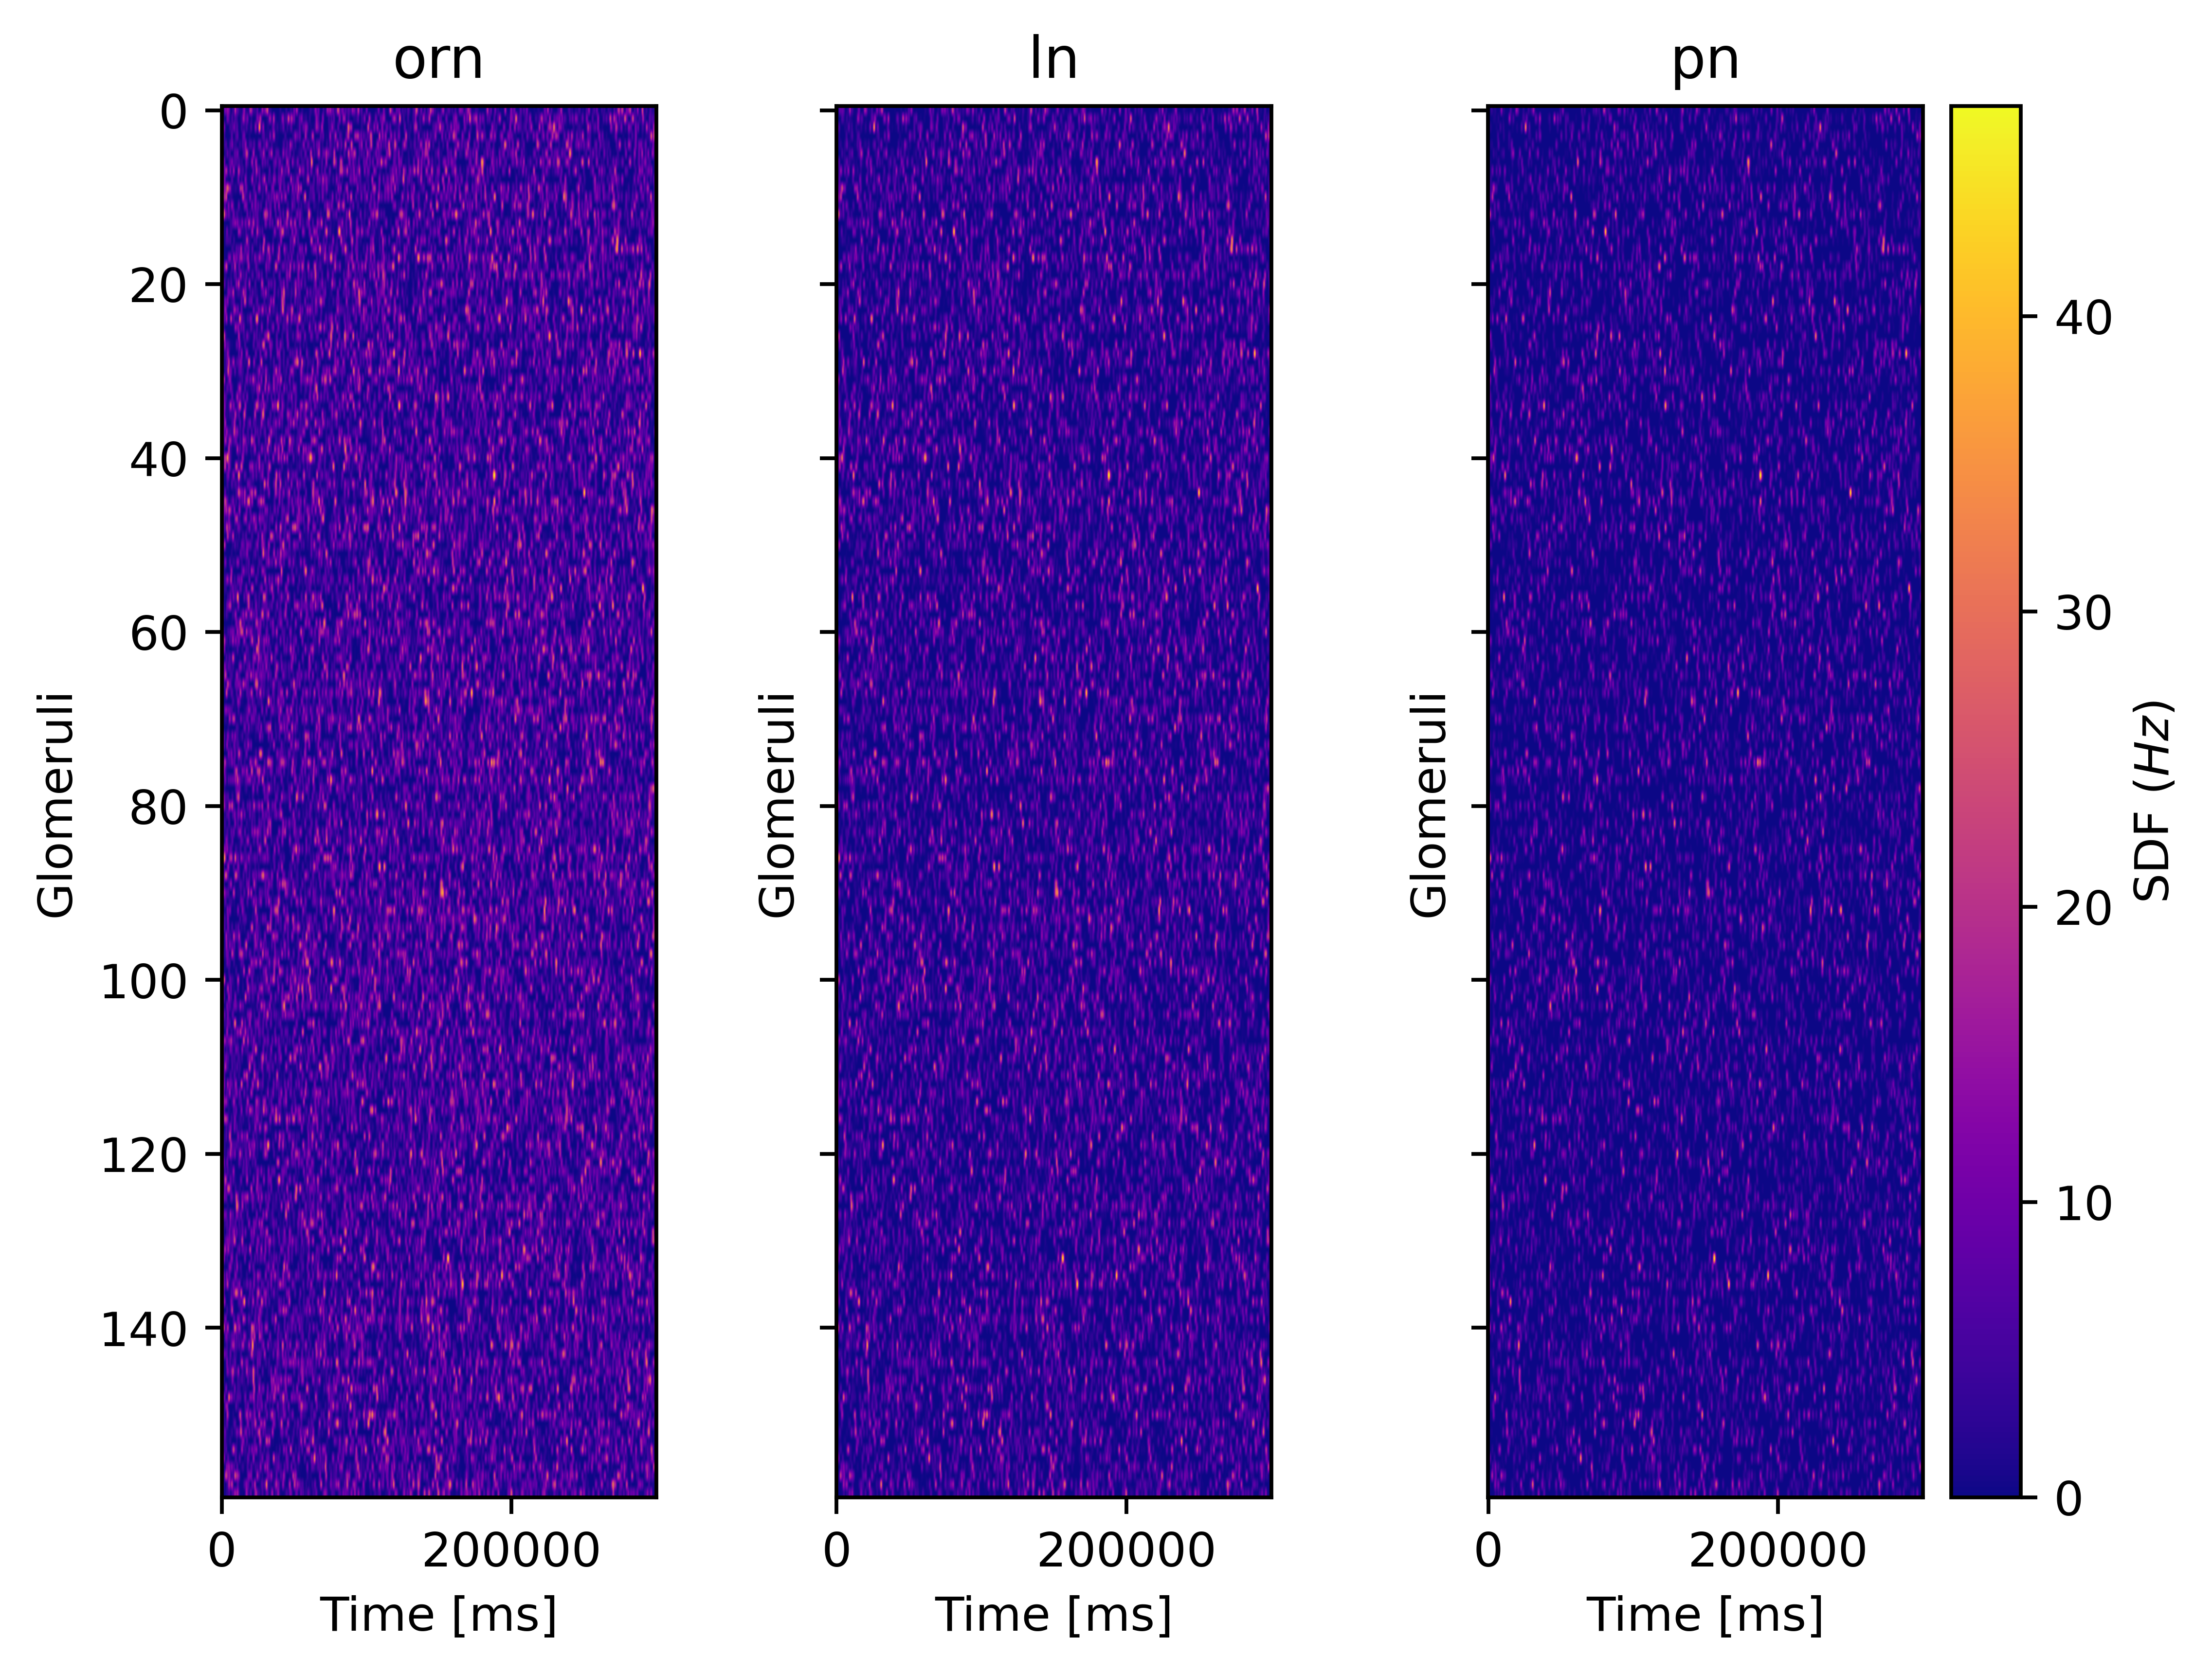
\includegraphics[width=\textwidth]{neuron-no-odor-sdf}
    \caption{$60$ seconds of spontaneous activity of neurons with no odor input. From left to right spike density matrix for olfactory receptor neurons, local neurons and projection neurons averaged over glomeruli.}
    \label{fig:neuron-no-odor-sdf}
  \end{figure}

  A better way to visualize this is through the spike density matrix, as in figure \ref{fig:neuron-no-odor-sdf}.
  This figure shows the average firing rate of a glomerulus divided by neuron population.
  It can be seen how the firing rate is similar across glomeruli since no olfactory receptor is activated by an odor.

  \begin{figure}
    \centering
    \includegraphics[width=\textwidth]{neuron-odor}
    \caption{$6$ seconds of activity of neurons with an odor presented to the network at $3$ second. From top to bottom: activation rate for an olfactory receptor, membrane potential of a random olfactory receptor neuron connected to the olfactory receptor, time series of the spike for the ORN. Time $[\SI{}{\milli\second}]$ on the $x$-axis}
    \label{fig:neuron-odor}
  \end{figure}

  The fact that the firing rate increases with the activity of the olfactory receptor can be better appreciated in figure \ref{fig:neuron-odor}: when the odor is presented at second $3$ the activity of the corresponding ORN increases significantly.

  \begin{figure}
    \centering
    \includegraphics[width=\textwidth]{neuron-odor-sdf}
    \caption{$3$ seconds of activity of neurons with an odor presented to the network during all the $3$ seconds.}
    \label{fig:neuron-odor-sdf}
  \end{figure}

  This can be further noticed by looking at the spike density matrix (figure \ref{fig:neuron-odor-sdf}).
  The figure shows how the glomerulus activated by this particular odor is much more active than the other.
  The activity of the network shows an initial increase in firing rate before it reaches an equilibrium.\\
  The parameters for the neurons are shown in table \ref{tab:neuron-parameters}.

  \begin{table}
    \centering
    \begin{tabular}{ c c | c c | c c }
      \hline
      \multicolumn{2}{c}{Olfactory receptor neurons} & \multicolumn{2}{c}{Projection neurons} & \multicolumn{2}{c}{Local neurons} \\
      \hline
      Parameter & Value & Parameter & Value & Parameter & Value \\
      $C$ & $\SI{1}{\milli\farad}$ & $C$ & $\SI{1}{\milli\farad}$ & $C$ & $\SI{1}{\milli\farad}$ \\
      $V_{reset}$ & $\SI{-70}{\milli\volt}$ & $V_{reset}$ & $\SI{-70}{\milli\volt}$ & $V_{reset}$ & $\SI{-70}{\milli\volt}$ \\
      $V_{thresh}$ & $\SI{-40}{\milli\volt}$ & $V_{thresh}$ & $\SI{-40}{\milli\volt}$ & $V_{thresh}$ & $\SI{-40}{\milli\volt}$ \\
      $V_{leak}$ & $\SI{-60}{\milli\volt}$ & $V_{leak}$ & $\SI{-60}{\milli\volt}$ & $V_{leak}$ & $\SI{-60}{\milli\volt}$ \\
      $V_{adapt}$ & $\SI{-70}{\milli\volt}$ & $V_{adapt}$ & $\SI{-70}{\milli\volt}$ & $V_{adapt}$ & $\SI{-70}{\milli\volt}$ \\
      $g_{leak\ 0}$ & $\SI{0.01}{\siemens}$ & $g_{leak\ 0}$ & $\SI{0.01}{\siemens}$ & $g_{leak\ 0}$ & $\SI{0.01}{\siemens}$ \\
      $g_{adapt\ 0}$ & $\SI{0.0015}{\siemens}$ & $g_{adapt\ 0}$ & $\SI{0.0015}{\siemens}$ & $g_{adapt\ 0}$ & $\SI{0.0015}{\siemens}$ \\
      $r_{scale}$ & $10$ & $r_{scale}$ & $10$ & $r_{scale}$ & $10$ \\
      $\tau_{adapt}$ & $\SI{1000}{\milli\second}$ & $\tau_{adapt}$ & $\SI{1000}{\milli\second}$ & $\tau_{adapt}$ & $\SI{1000}{\milli\second}$ \\
      $T_{ref}$ & $\SI{36}{\celsius}$ & $T_{ref}$ & $\SI{36}{\celsius}$ & $T_{ref}$ & $\SI{36}{\celsius}$ \\
      $T$ & $\SI{30}{\celsius}$ & $T$ & $\SI{30}{\celsius}$ & $T$ & $\SI{30}{\celsius}$ \\
      $Q$ & $1.1$ & $Q$ & $1.1$ & $Q$ & $1.1$ \\
      $\sigma$ & $\frac{1.4}{\sqrt{dt}}$ & $\sigma$ & $\frac{1.4}{\sqrt{dt}}$ & $\sigma$ & $\frac{1.4}{\sqrt{dt}}$ \\
      \hline
    \end{tabular}
    \caption{Parameters for the neurons.}
    \label{tab:neuron-parameters}
  \end{table}

  \subsection{Synapses}
  The model has two types of synapses:

  \begin{multicols}{2}
    \begin{itemize}
      \item Excitatory.
      \item Inhibitory.
    \end{itemize}
  \end{multicols}

  Both are modeled as conductance-based synapses according to the static pulse model with an exponential decay as in equations \ref{eqs:static-pulse} and \ref{eqs:exponential-decay}.
  There are two differences in how the inhibitory and excitatory synapses are modeled.

    \subsubsection{Excitatory synapses}
    Excitatory synapses form sparse directional connections between:

    \begin{itemize}
      \item Olfactory receptor neurons and projection neurons.
      \item Olfactory receptor neurons and local neurons.
      \item Projection neurons and local neurons.
    \end{itemize}

    Where each neuron of the source population is connected with a random neuron of the target population.

    \begin{figure}
      \centering
      \includegraphics[width=\textwidth]{excitatory-synapses-conductance}
      \caption{Behavior of the conductance of an excitatory synapse (bottom) in relation to the activity of the presynaptic neuron (top).}
      \label{fig:excitatory-synapses-conductance}
    \end{figure}

    The behavior of the model on the changes in conductance in relation to the activity of the presynaptic neuron can be seen in figure \ref{fig:excitatory-synapses-conductance}.
    It can be seen how the more the presynaptic neuron spikes the faster this conductance increases, facilitating the ability of the postsynaptic neuron to spike.\\
    The parameters for the excitatory conductances are found in table \ref{tab:excitatory-synapses-parameters}.

    \begin{table}
      \centering
      \begin{tabular}{ c c | c c | c c }
        \hline
        \multicolumn{2}{c}{ORN to PN} & \multicolumn{2}{c}{ORN to LN} & \multicolumn{2}{c}{PN to LN} \\
        \hline
        Parameter & Value & Parameter & Value & Parameter & Value \\
        $g$ & $\SI{0.008}{\siemens}$ & $g$ & $\SI{0.008}{\siemens}$ & $g$ & $\SI{0.001}{\siemens}$ \\
        $E$ & $\SI{0}{\milli\volt}$ & $E$ & $\SI{0}{\milli\volt}$ & $E$ & $\SI{0}{\milli\volt}$ \\
        $\tau$ & $\SI{10}{\milli\second}$ & $\tau$ & $\SI{10}{\milli\second}$ & $\tau$ & $\SI{10}{\milli\second}$ \\
        \hline
      \end{tabular}
      \caption{Parameters for the excitatory synapses.}
      \label{tab:excitatory-synapses-parameters}
    \end{table}

    \subsubsection{Inhibitory synapses}
    Inhibitory synapses form dense directional connections between:

    \begin{itemize}
      \item Local neurons and projection neurons.
      \item Local neurons and local neurons.
    \end{itemize}

    Where each neuron of the source population is connected with all the neurons of the target population.

    \begin{figure}
      \centering
      \includegraphics[width=\textwidth]{inhibitory-synapses-conductance}
      \caption{Behavior of the conductance of an inhibitory synapse (bottom) in relation to the activity of the presynaptic neuron (top).}
      \label{fig:inhibitory-synapses-conductance}
    \end{figure}

    The behavior of the model on the changes in conductance in relation to the activity of the presynaptic neuron can be seen in figure \ref{fig:inhibitory-synapses-conductance}.
    It can be seen how the more the presynaptic neuron spikes the faster the conductance decreases, making it harder for the postsynaptic neuron to spike.\\
    The parameters for the inhibitory conductances are found in table \ref{tab:inhibitory-synapses-parameters}.

    \begin{table}
      \centering
      \begin{tabular}{ c c | c c }
        \hline
        \multicolumn{2}{c}{LN to PN} & \multicolumn{2}{c}{LN to LN}\\
        \hline
        Parameter & Value & Parameter & Value\\
        $g$ & $\SI{5.5e-5}{\siemens}$ & $g$ & $\SI{2.0e-5}{\siemens}$\\
        $E$ & $\SI{-80}{\milli\volt}$ & $E$ & $\SI{-80}{\milli\volt}$\\
        $\tau$ & $\SI{20}{\milli\second}$ & $\tau$ & $\SI{20}{\milli\second}$\\
        \hline
      \end{tabular}
      \caption{Parameters for the inhibitory synapses.}
      \label{tab:inhibitory-synapses-parameters}
    \end{table}



\section{Response to odours}
As described in section \ref{sec:odors}, the odors are described as Gaussian profiles, determining the ability of the molecule to bind each of the $160$ olfactory receptors.
Because of these odors are described by four parameters:

\begin{itemize}
  \item $c$: the concentration of the odor.
  \item $x$ or the midpoint: the olfactory receptor where the mean of the Gaussian profile is located.
  \item $A$: the amplitude of the profile, determining the maximum value of the profile.
  \item $\sigma$: the standard deviation of the profile, determining the width of the profile.
\end{itemize}

Besides two odors for which this Gaussian profile was already determined in \cite{data-driven-antennal-lobe-model}, $A$ and $\sigma$ are sampled from bounded Gaussian distributions.

\begin{table}
  \centering
  \begin{tabular}{ c c c }
    \hline
    & $A$ & $\sigma$ \\
    \hline
    Isoamyl acetate & $0.8$ & $3$\\
    Geosmin & $4.4$ & $10$\\
    Other & $x\sim\mathcal{N}(1.5,0.5): x \in [0, 4.0]$ & $x\sim\mathcal{N}(3,0.5): x \in [1.5, \infty[$\\
    \hline
  \end{tabular}
  \caption{Parameters for the odors.}
  \label{tab:odors}
\end{table}

A full list of odor parameters can be found in table \ref{tab:odors}.
It can be noted that the isoamyl acetate (IAA) has a lower standard deviation than geosmin, meaning that it will tend to activate less olfactory receptors than geosmin.\\

\begin{figure}
  \centering
  \includegraphics[width=\textwidth]{iaa}
  \caption{Spike density matrix of the antennal lobe in response to isoamyl acetate (concentration $\SI{e-3}{\mole\per\litre}$). $\SI{3}{\second}$ of simulation.}
  \label{fig:iaa}
\end{figure}

\begin{figure}
  \centering
  \includegraphics[width=\textwidth]{geosmin}
  \caption{Spike density matrix of the antennal lobe in response to geosmin (concentration $\SI{e-3}{\mole\per\litre}$). $\SI{3}{\second}$ of simulation.}
  \label{fig:geosmin}
\end{figure}

The response of the network to IAA and geosmin can be seen respectively in figures \ref{fig:iaa} and \ref{fig:geosmin}.
It can be noted how geosmin, thanks to its higher $\sigma$ activates more glomeruli, while IAA activates fewer glomeruli, but with a higher firing rate.
It is important to note that in this case both the temperature-dependent white noise and the Poisson trains were not included in the model, as done in \cite{bee-geosmin}.
They were excluded from this simulation as their impact on the firing rate of the neurons was not significant, and they were not necessary to reproduce the biological behavior with enough accuracy.

\section{Awake state}
The awake state is represented by the model described in section \ref{sec:behavior-components}.
The parameters for the neurons are the ones in \ref{tab:neuron-parameters}, while the parameters for the synapses are the ones in \ref{tab:excitatory-synapses-parameters} and in \ref{tab:inhibitory-synapses-parameters}.
The model is left to evolve without any odor input, with only the temperature-dependent white noise.

\begin{figure}
  \centering
  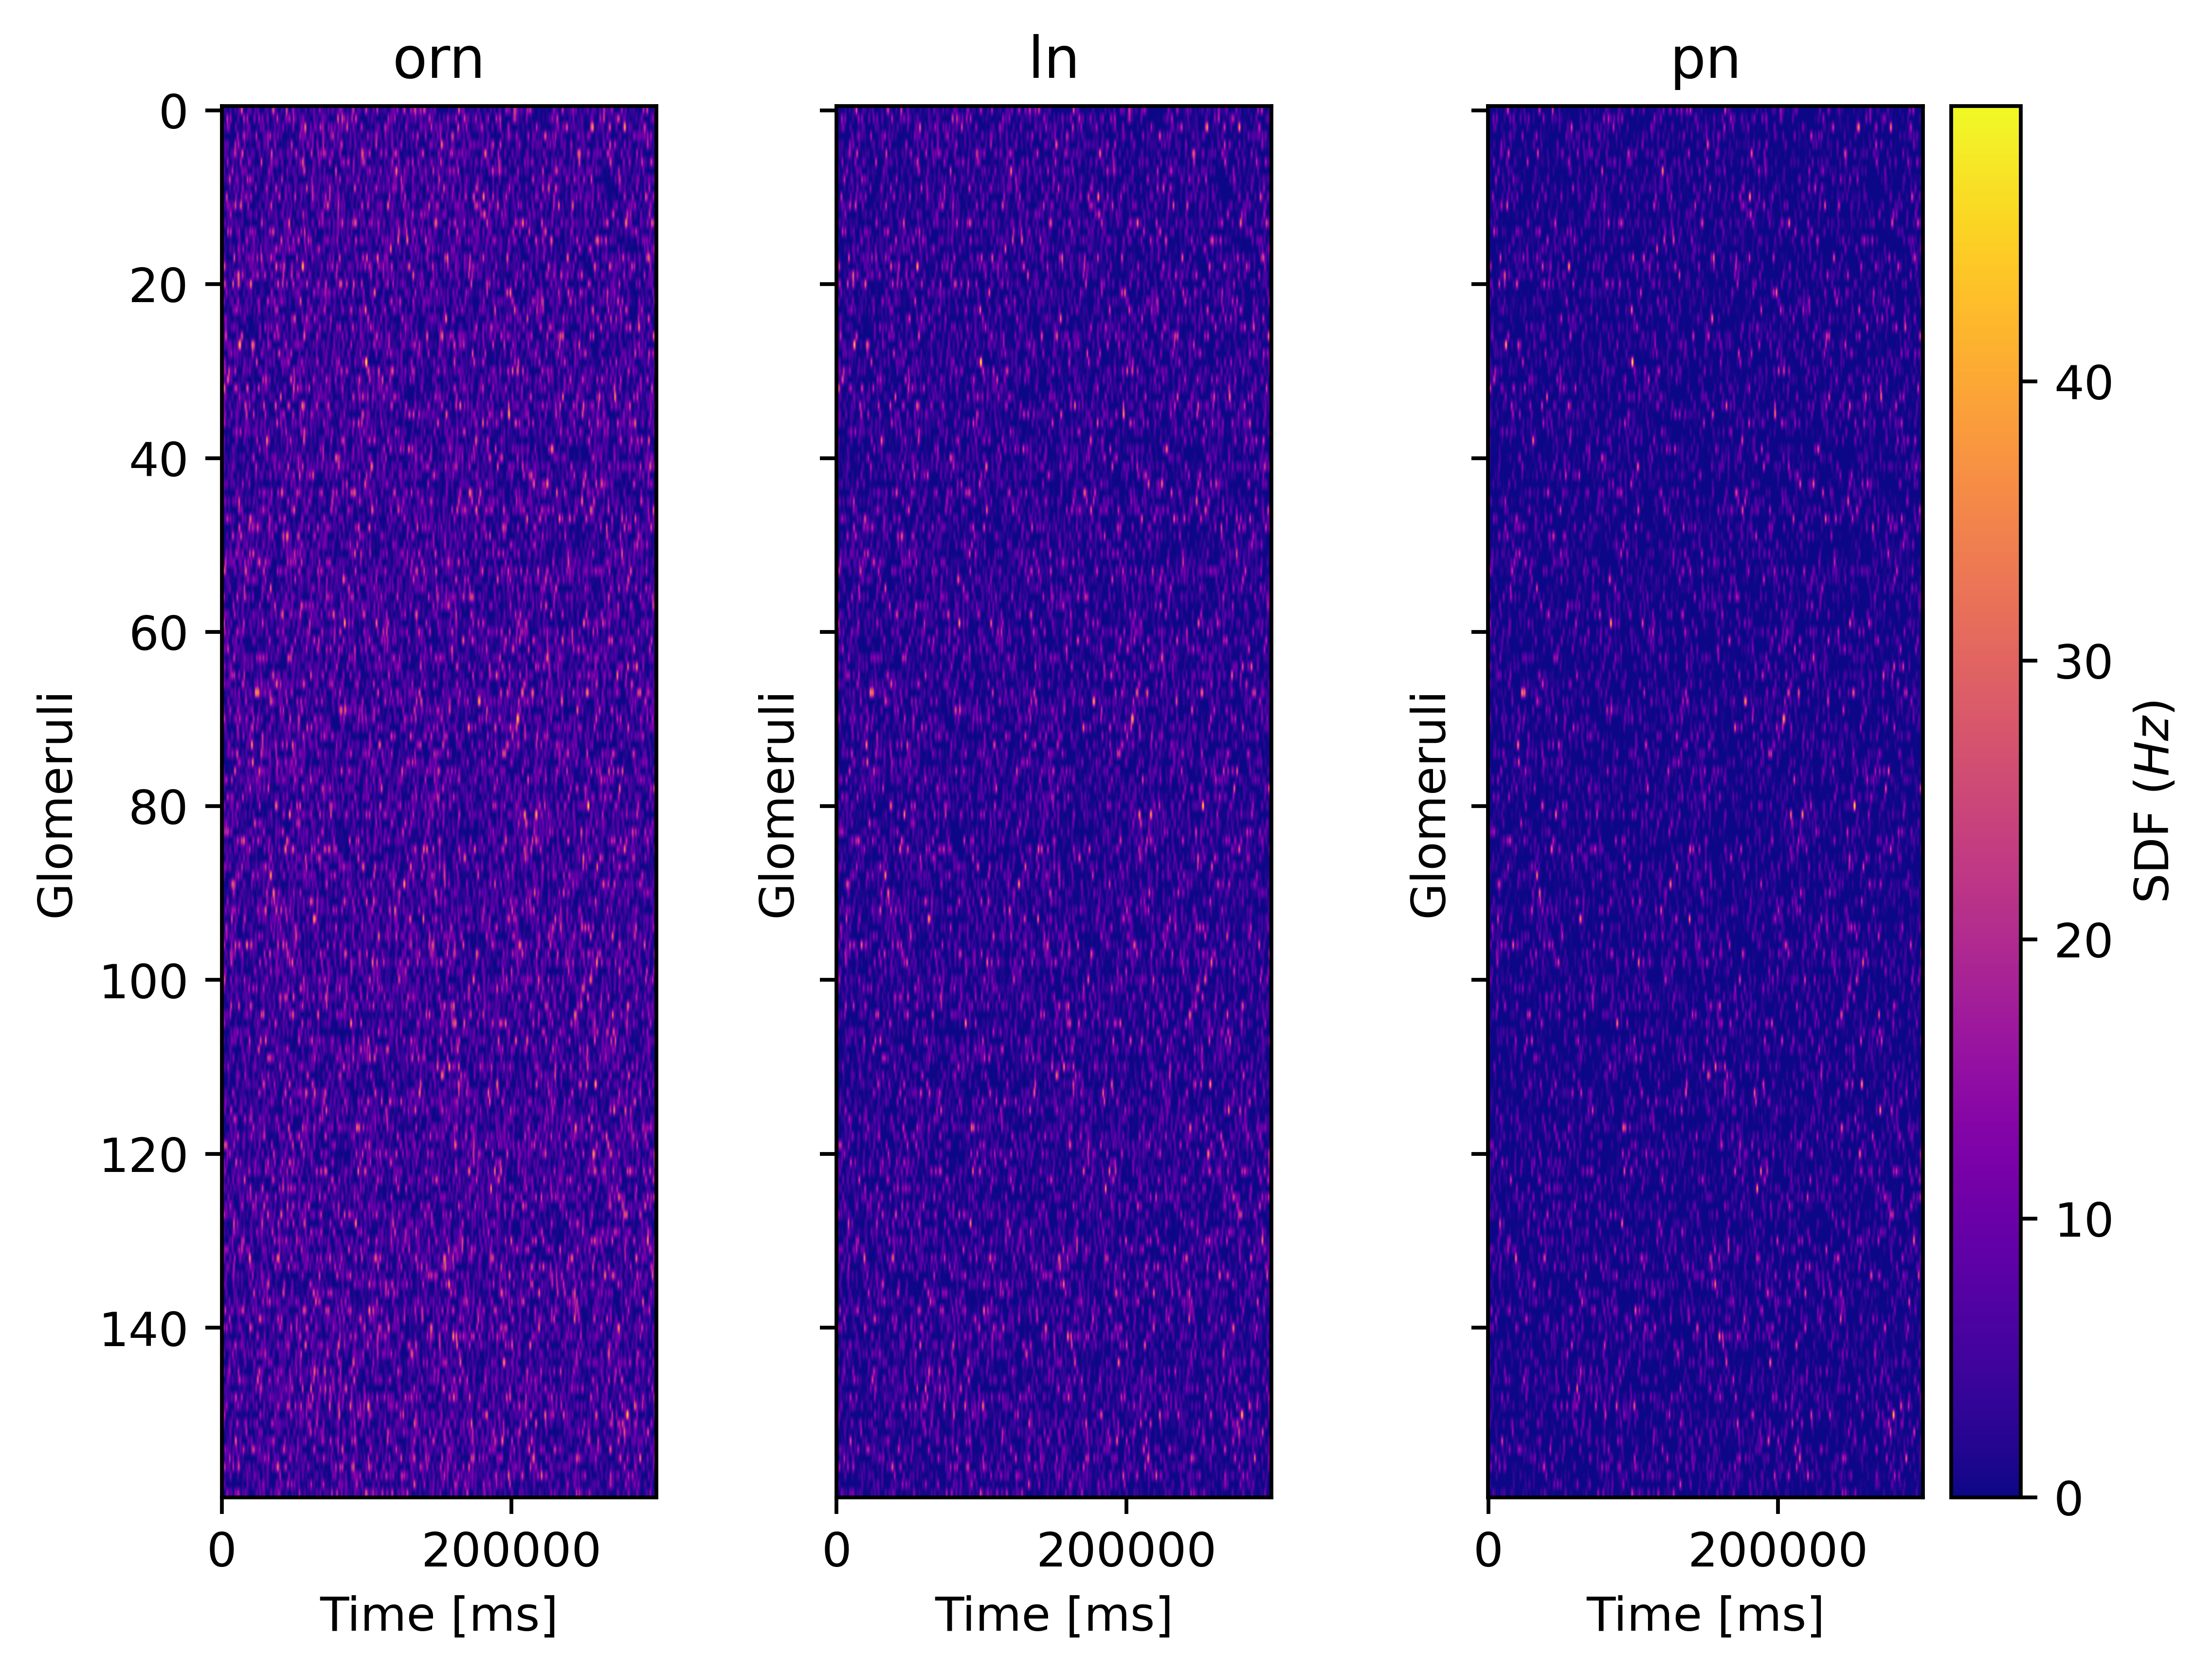
\includegraphics[width=\textwidth]{sdf-awake-no-poisson}
  \caption{Spike density matrix of the spontaneous activity of the antennal lobe without the Poisson trains. $\SI{60}{\second}$ of simulation.}
  \label{fig:sdf-awake-no-poisson}
\end{figure}

Figure \ref{fig:sdf-awake-no-poisson} shows the activity of the glomeruli in the awake state without the Poisson trains.
It is visible the effect of the inhibitory synapses on the projection neurons, as the average firing rate of the projection neurons is lower than the one of the olfactory receptor neurons.

\begin{figure}
  \centering
  \includegraphics[width=\textwidth]{correlation-awake-no-poisson}
  \caption{Correlation of the spontaneous activity of the antennal lobe without the Poisson trains. $\SI{60}{\second}$ of simulation. Average correlation per population $\overline{Corr_{ORN}} = 0.007$, $\overline{Corr_{LN}} = 0.003$, $\overline{Corr_{PN}} = 0.001$.}
  \label{fig:correlation-awake-no-poisson}
\end{figure}

Figure \ref{fig:correlation-awake-no-poisson} shows the correlation between the glomeruli in the awake state without the Poisson trains.
It can be seen how the correlation in the projection neurons tends to be lower than the one in the olfactory receptor neurons, due to the inhibitory synapses that decouple the projection neurons from the input in the olfactory receptor neurons.

  \subsection{Adding the Poisson trains}
  The Poisson trains are added to the model, to explore what is the effect of a correlated input on the activity of the antennal lobe.

  \begin{figure}
    \centering
    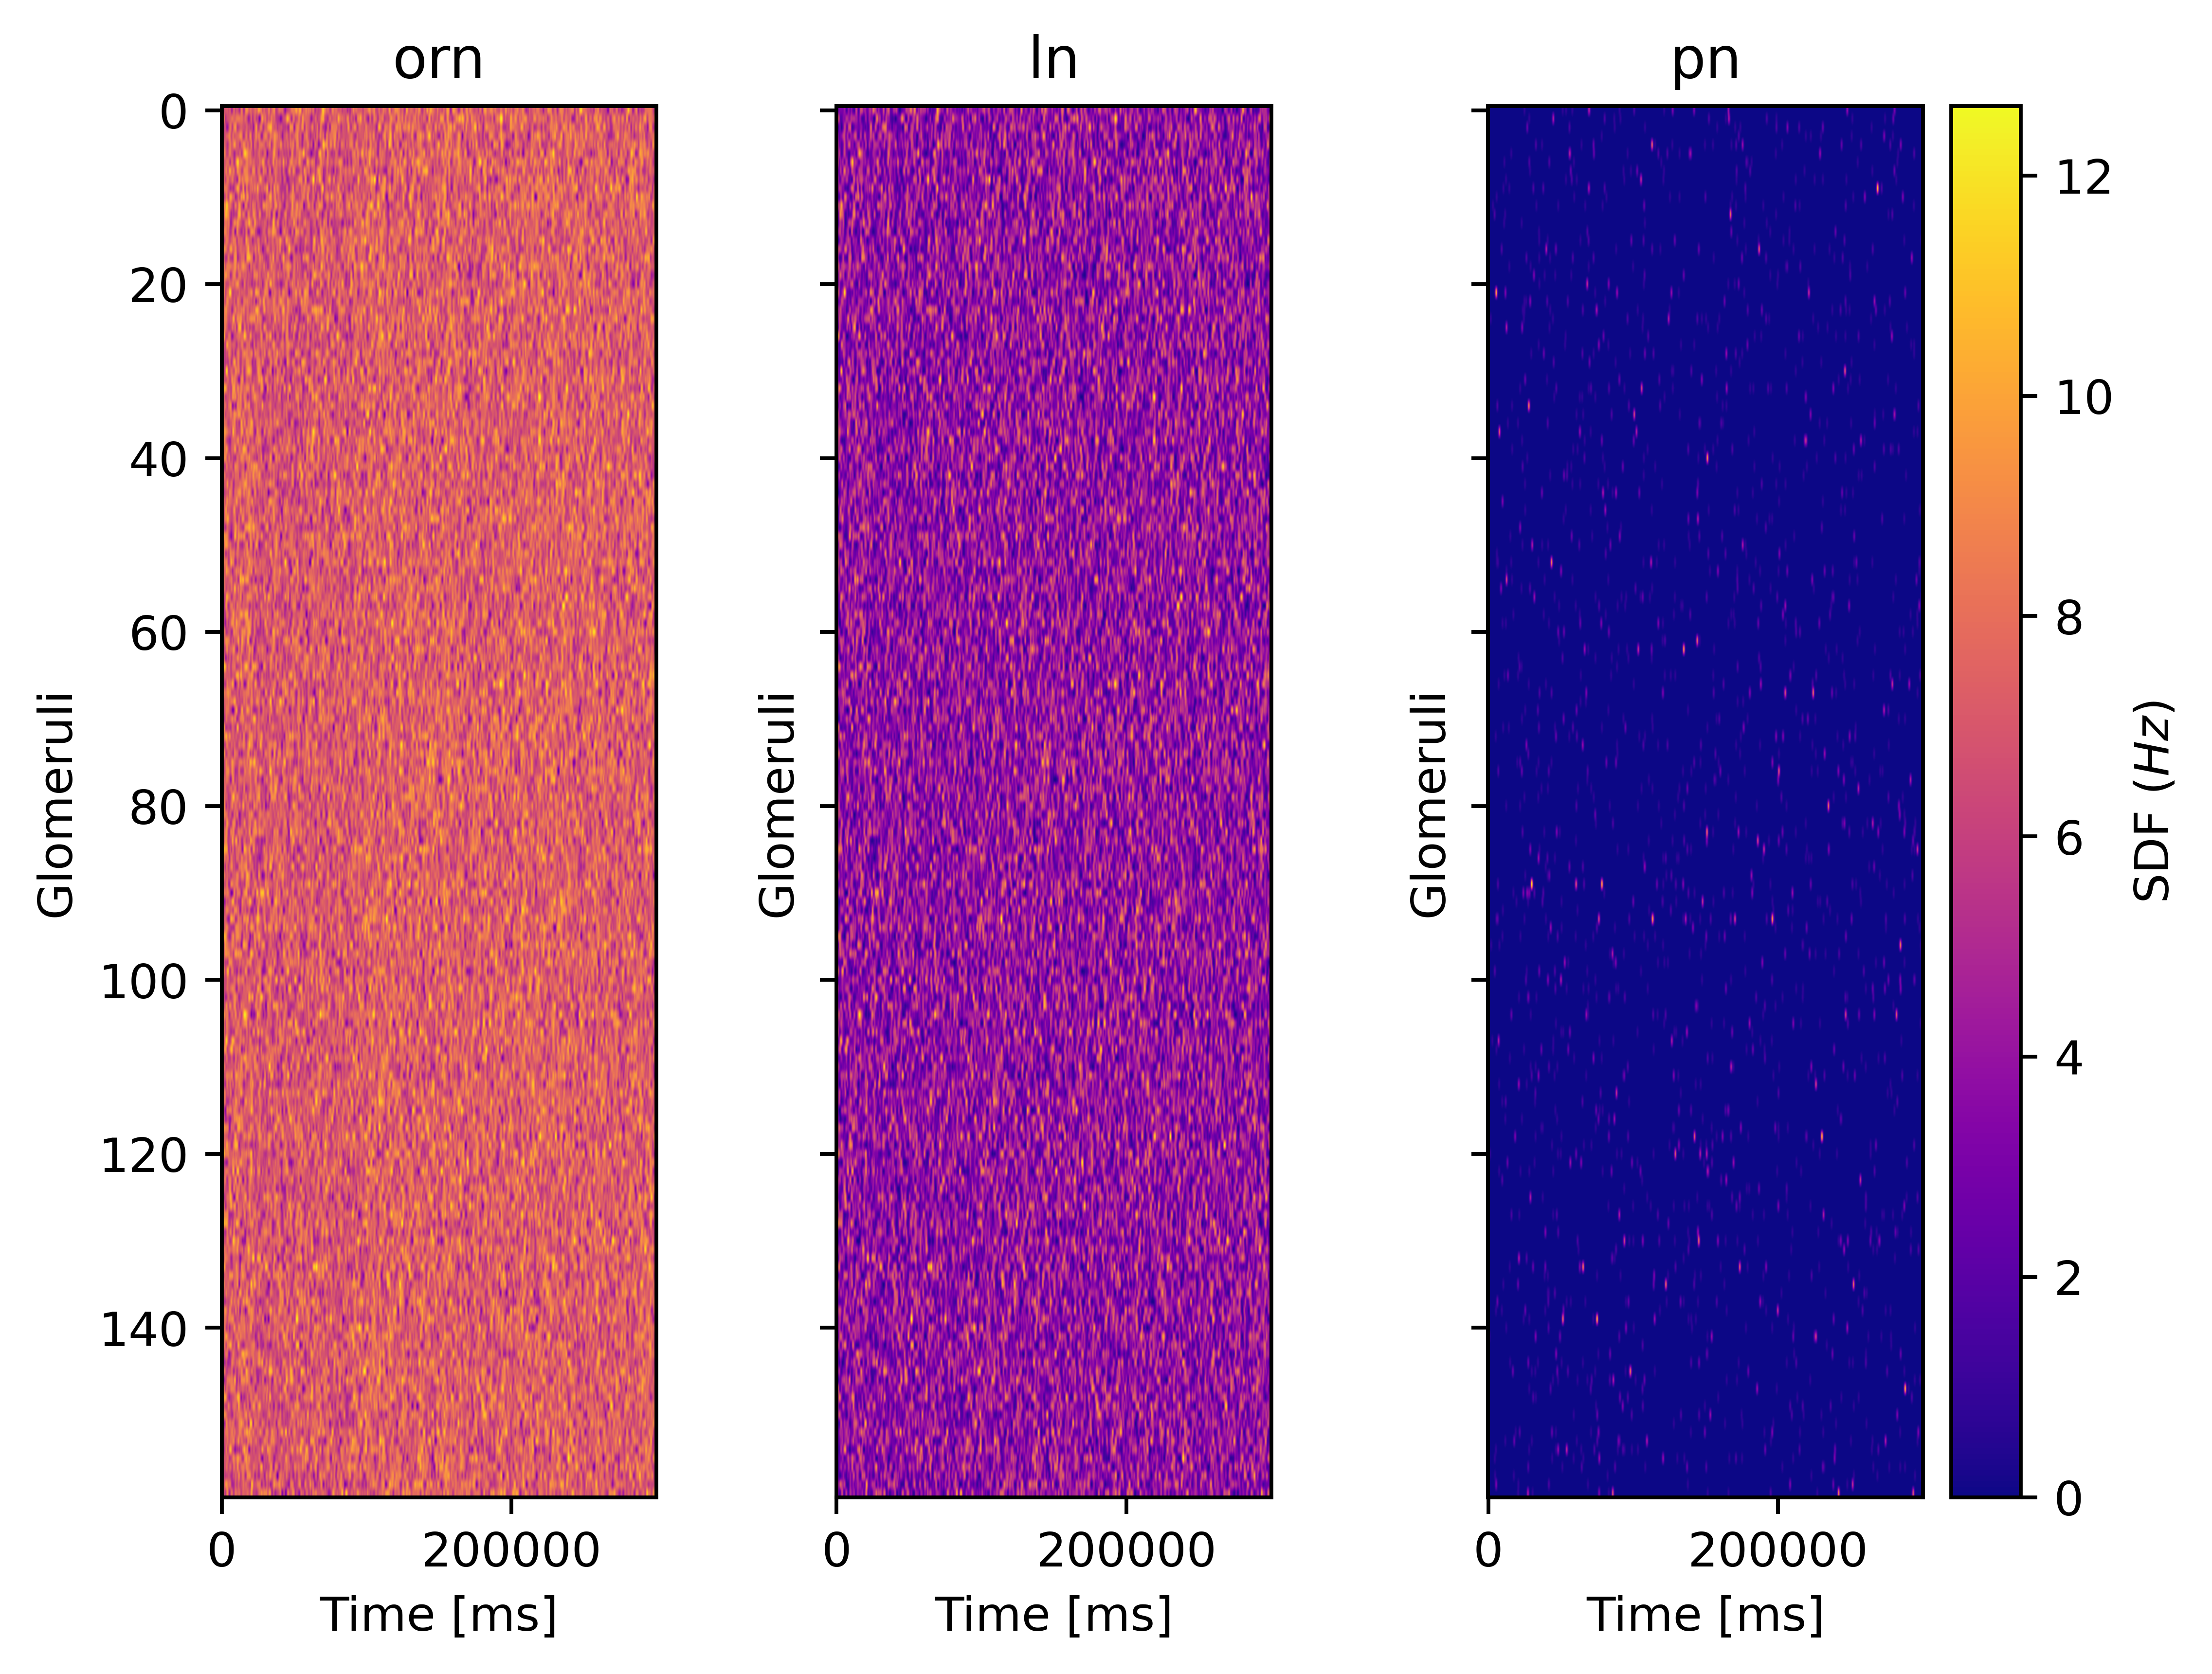
\includegraphics[width=\textwidth]{sdf-awake-poisson}
    \caption{Spike density matrix of the spontaneous activity of the antennal lobe with the Poisson trains. $\SI{60}{\second}$ of simulation.}
    \label{fig:sdf-awake-poisson}
  \end{figure}

  The Poisson trains have a strong effect on the activity of the antennal lobe, as shown in figure \ref{fig:sdf-awake-poisson}.
  It can be seen that when Poisson trains are added, although the firing rate of the olfactory receptor neurons doesn't change, the activity of the projection neurons goes almost completely to zero.\\
  This is due to the strong synaptic inhibition that the projection neurons receive from the local neurons: the decoupling effect of the inhibitory part of the system is too strong to allow for activity in the projection neurons and seems to have a much greater effect when the output coming from the olfactory receptor neurons is correlated.

  \begin{figure}
    \centering
    \includegraphics[width=\textwidth]{correlation-awake-poisson}
    \caption{Correlation of the spontaneous activity of the antennal lobe with the Poisson trains. $\SI{60}{\second}$ of simulation. Average correlation per population $\overline{Corr_{ORN}} = 0.04$, $\overline{Corr_{LN}} = 0.006$, $\overline{Corr_{PN}} = 0.007$}
    \label{fig:correlation-awake-poisson}
  \end{figure}

  At the same time due to the inhibitory effect of the local neurons, the correlation between the projection neurons across glomeruli is higher than the system without the correlated input.
  This is not due to the correlation present in the input, but rather due to the fact that the activity of the projection neurons becomes so inhibited that its correlation increases: neurons that never fire have a completely correlated activity.
  This is further supported by the fact that this is the only simulation where the correlation of the projection neurons is higher than the one of the olfactory receptor neurons.
  Another evidence of this is the increased variability in the correlation of the Projection neurons (figure \ref{fig:correlation-awake-poisson}), suggesting that the activity of the projection neurons per glomerulus is more inhibited for those glomeruli that tend to receve as input more correlated Poisson trains.\\
  Moreover, this suggests that there is no correlated input in the awake state and that it can be found only in the asleep state.

\section{Asleep state}
Finding the correct parameters that describe the asleep state required two modifications from the awake state:

\begin{itemize}
  \item Introducing a correlated input in the form of Poisson trains.
  \item Reducing the strength of the inhibitory synapses.
\end{itemize}

The optimal Poisson trains were already found in \ref{sec:finding-poisson-train}, so the only thing left to explore is the effect of the inhibitory synapses on the coupling of the system.
To do so several simulations have been run with different reducing factors for the inhibitory synapses.
The new simulations with the corresponding value of the inhibitory synapses are shown in table \ref{tab:inhibitory-synapses-parameters-asleep}.

\begin{table}
  \centering
  \begin{tabular}{ c c c c c c }
    \hline
    & Awake & Halved & Quarter & Tenth & Hundredth \\
    \hline
    Reducing factor & $1$ & $0.5$ & $0.25$ & $0.1$ & $0.01$ \\
    $g_{LN \to LN}$ & $\SI{2.0e-5}{\siemens}$ & $\SI{1.0e-5}{\siemens}$ & $\SI{5.0e-6}{\siemens}$ & $\SI{2.0e-6}{\siemens}$ & $\SI{2.0e-7}{\siemens}$ \\
    $g_{LN \to PN}$ & $\SI{5.5e-5}{\siemens}$ & $\SI{2.75e-5}{\siemens}$ & $\SI{1.375e-5}{\siemens}$ & $\SI{5.5e-6}{\siemens}$ & $\SI{5.5e-7}{\siemens}$ \\
    \hline
  \end{tabular}
  \caption{Reduction of the inhibitory synapses to find the asleep state}
  \label{tab:inhibitory-synapses-parameters-asleep}
\end{table}

\begin{figure}
  \begin{subfigure}[t]{0.5\textwidth}
    \centering
    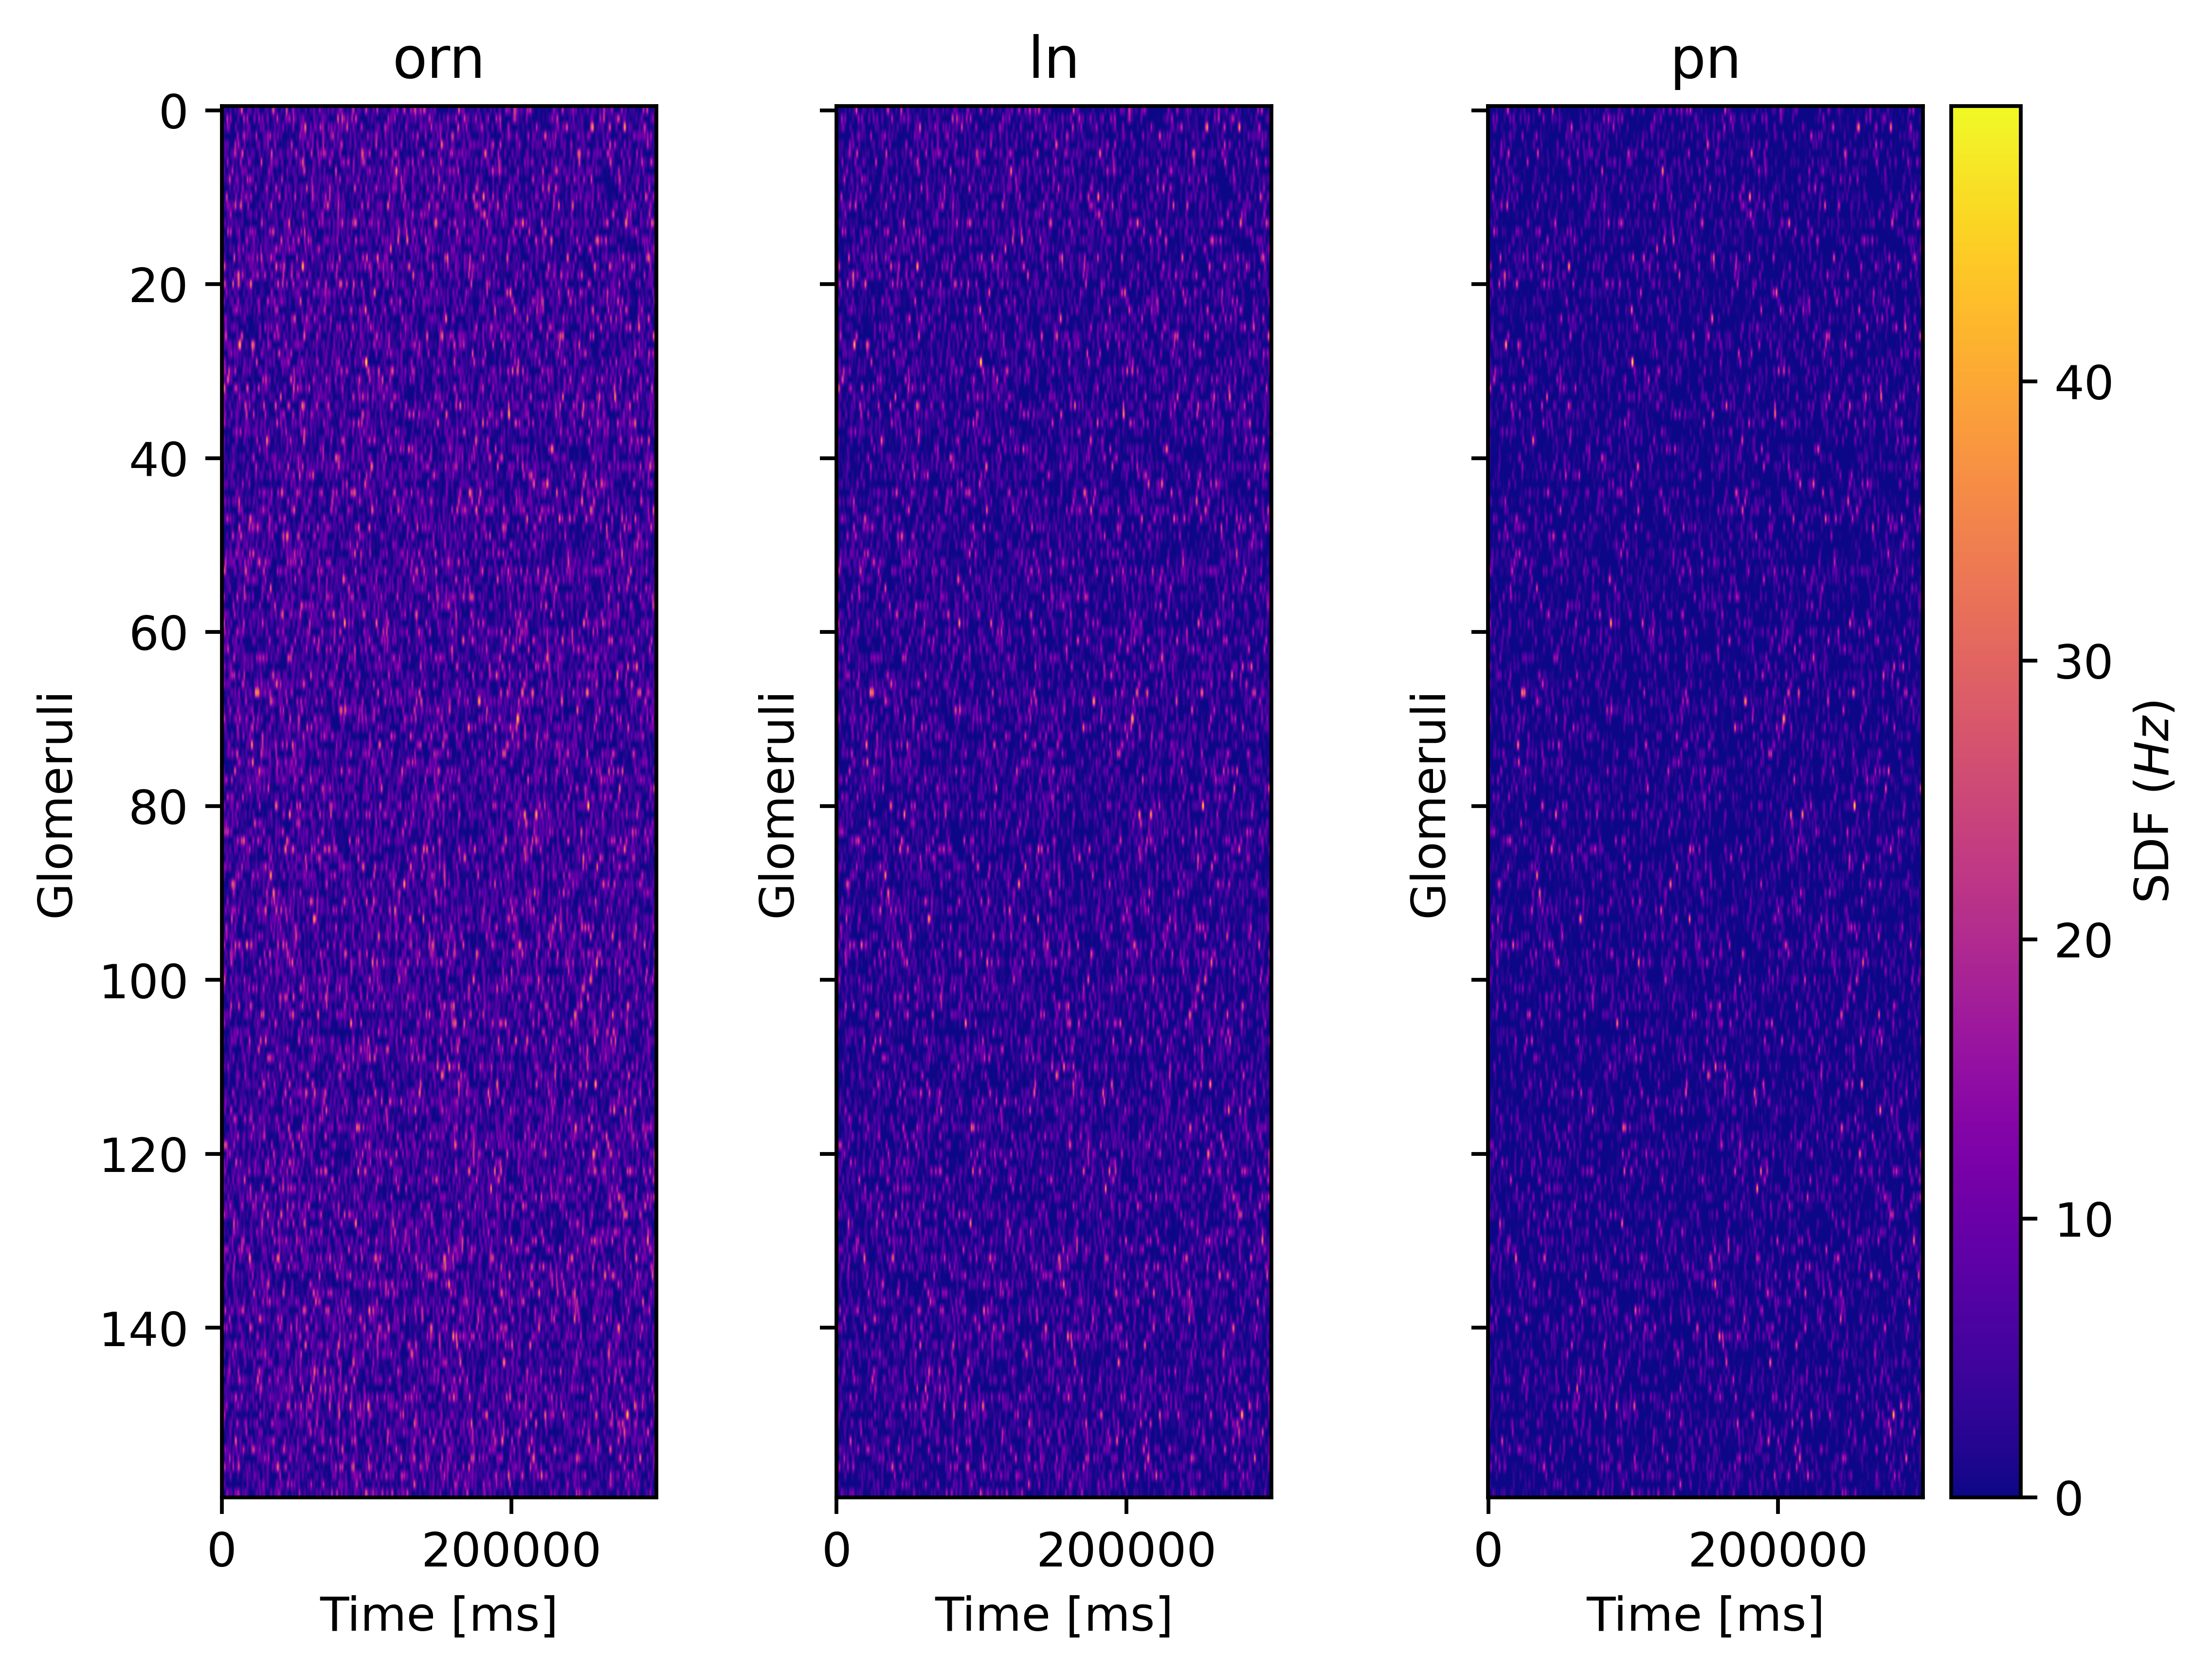
\includegraphics[width=\textwidth]{sdf-awake-no-poisson}
    \caption{Awake (without correlated input).}
    \label{fig:sdf-awake-poisson-finding-asleep}
  \end{subfigure}
  \begin{subfigure}[t]{0.5\textwidth}
    \centering
    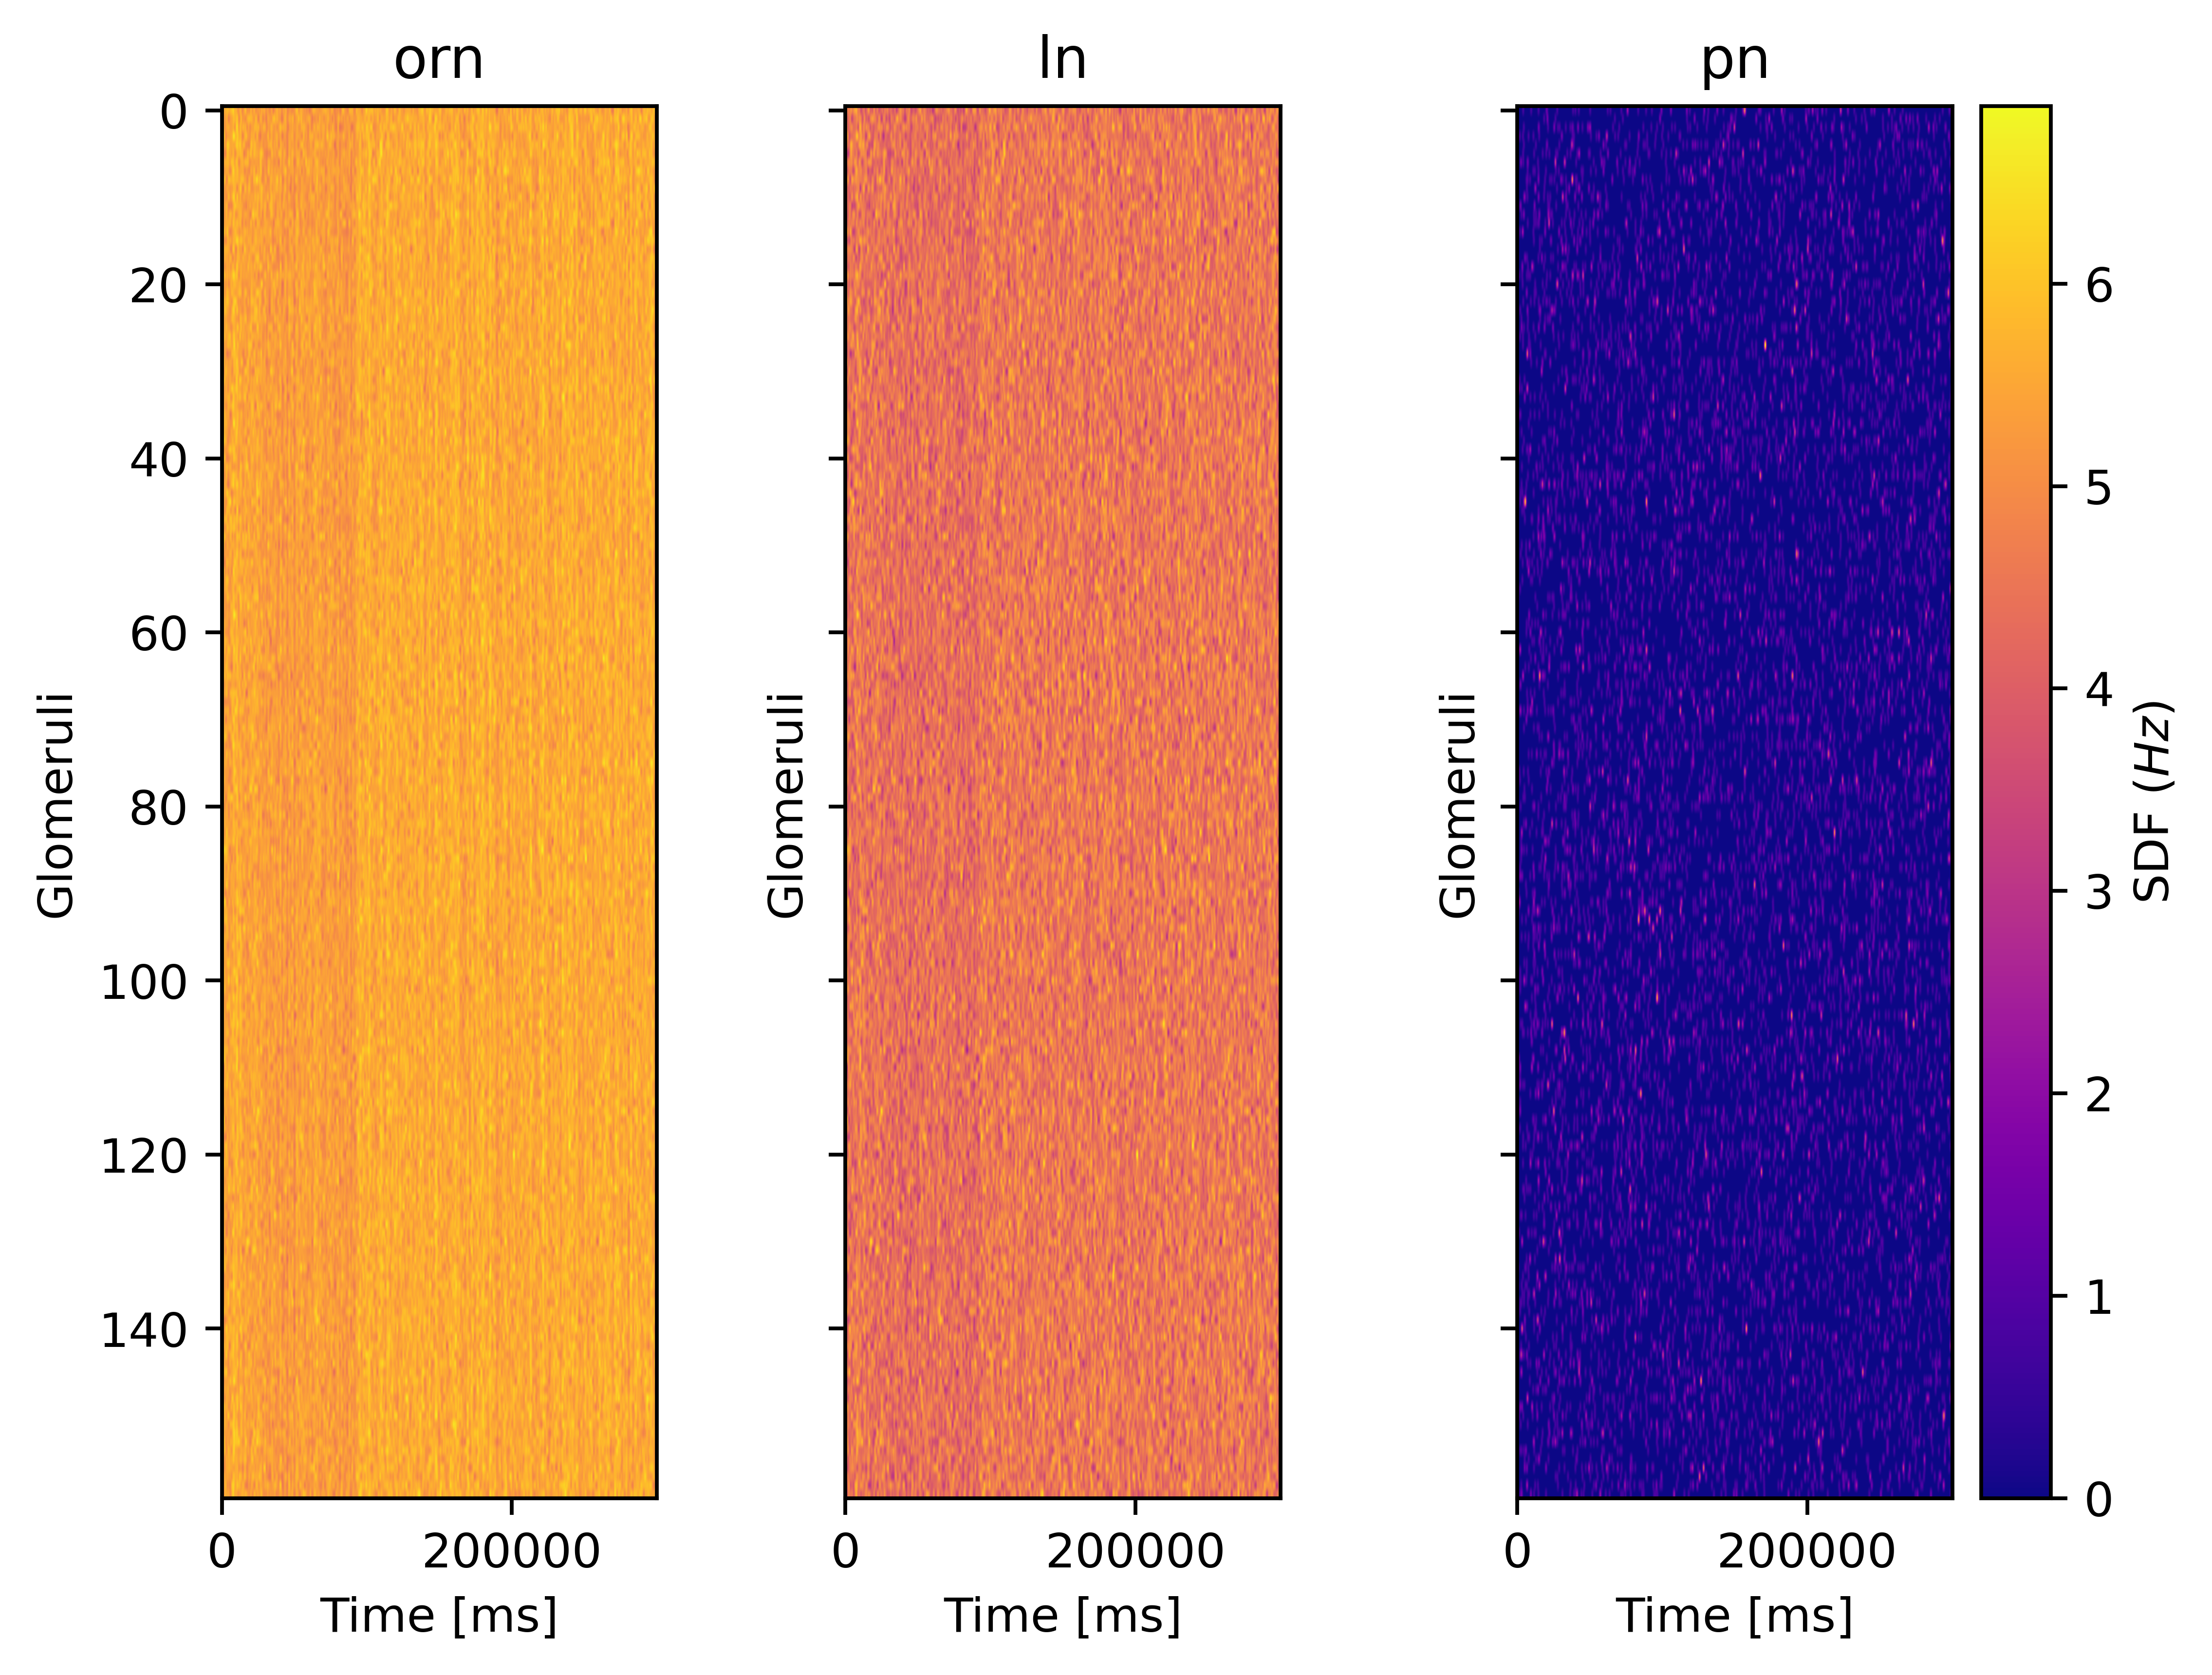
\includegraphics[width=\textwidth]{sdf-halved-poisson}
    \caption{Halved.}
    \label{fig:sdf-halved-poisson-finding-asleep}
  \end{subfigure}
  \begin{subfigure}[t]{\textwidth}
    \centering
    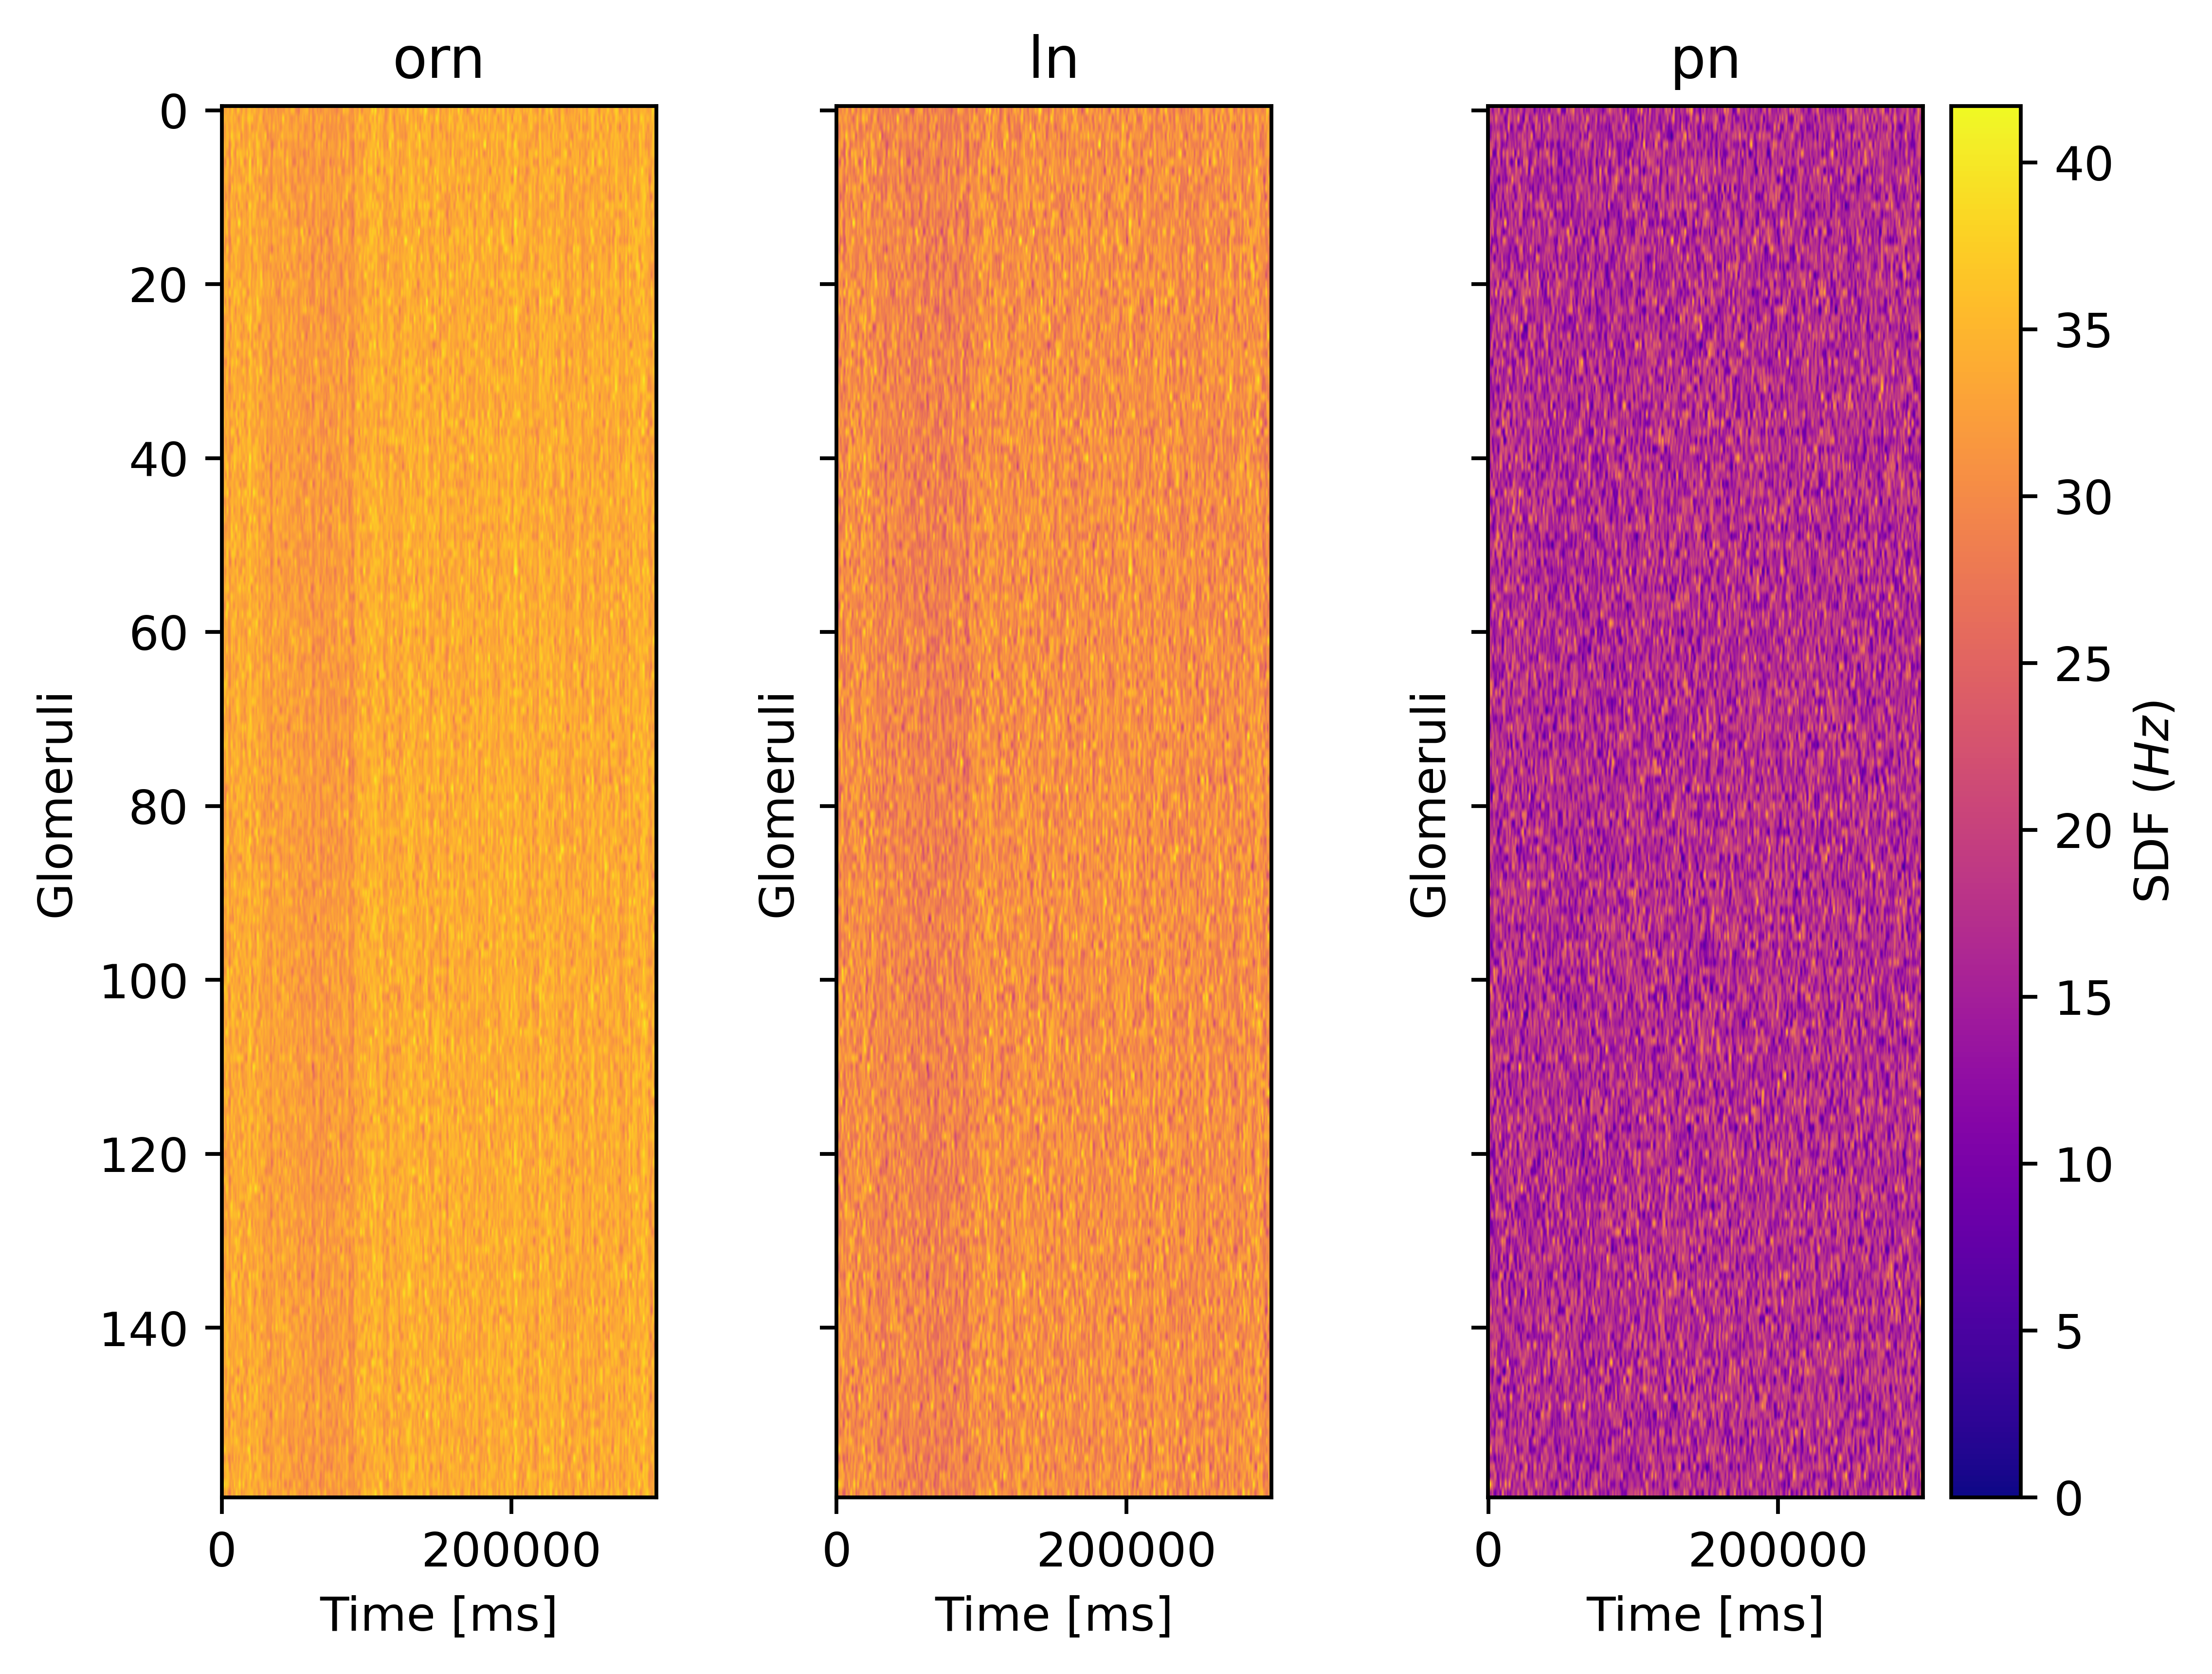
\includegraphics[width=0.5\textwidth]{sdf-quarter-poisson}
    \caption{Quarter.}
    \label{fig:sdf-quarter-poisson-finding-asleep}
  \end{subfigure}
  \caption{Spike density matrix of the spontaneous activity of the antennal lobe with the Poisson trains and different reduction of the inhibitory synapses. $\SI{60}{\second}$ of simulation.}
  \label{fig:sdf-finding-asleep-1}
\end{figure}

\begin{figure}
  \begin{subfigure}[t]{0.5\textwidth}
    \centering
    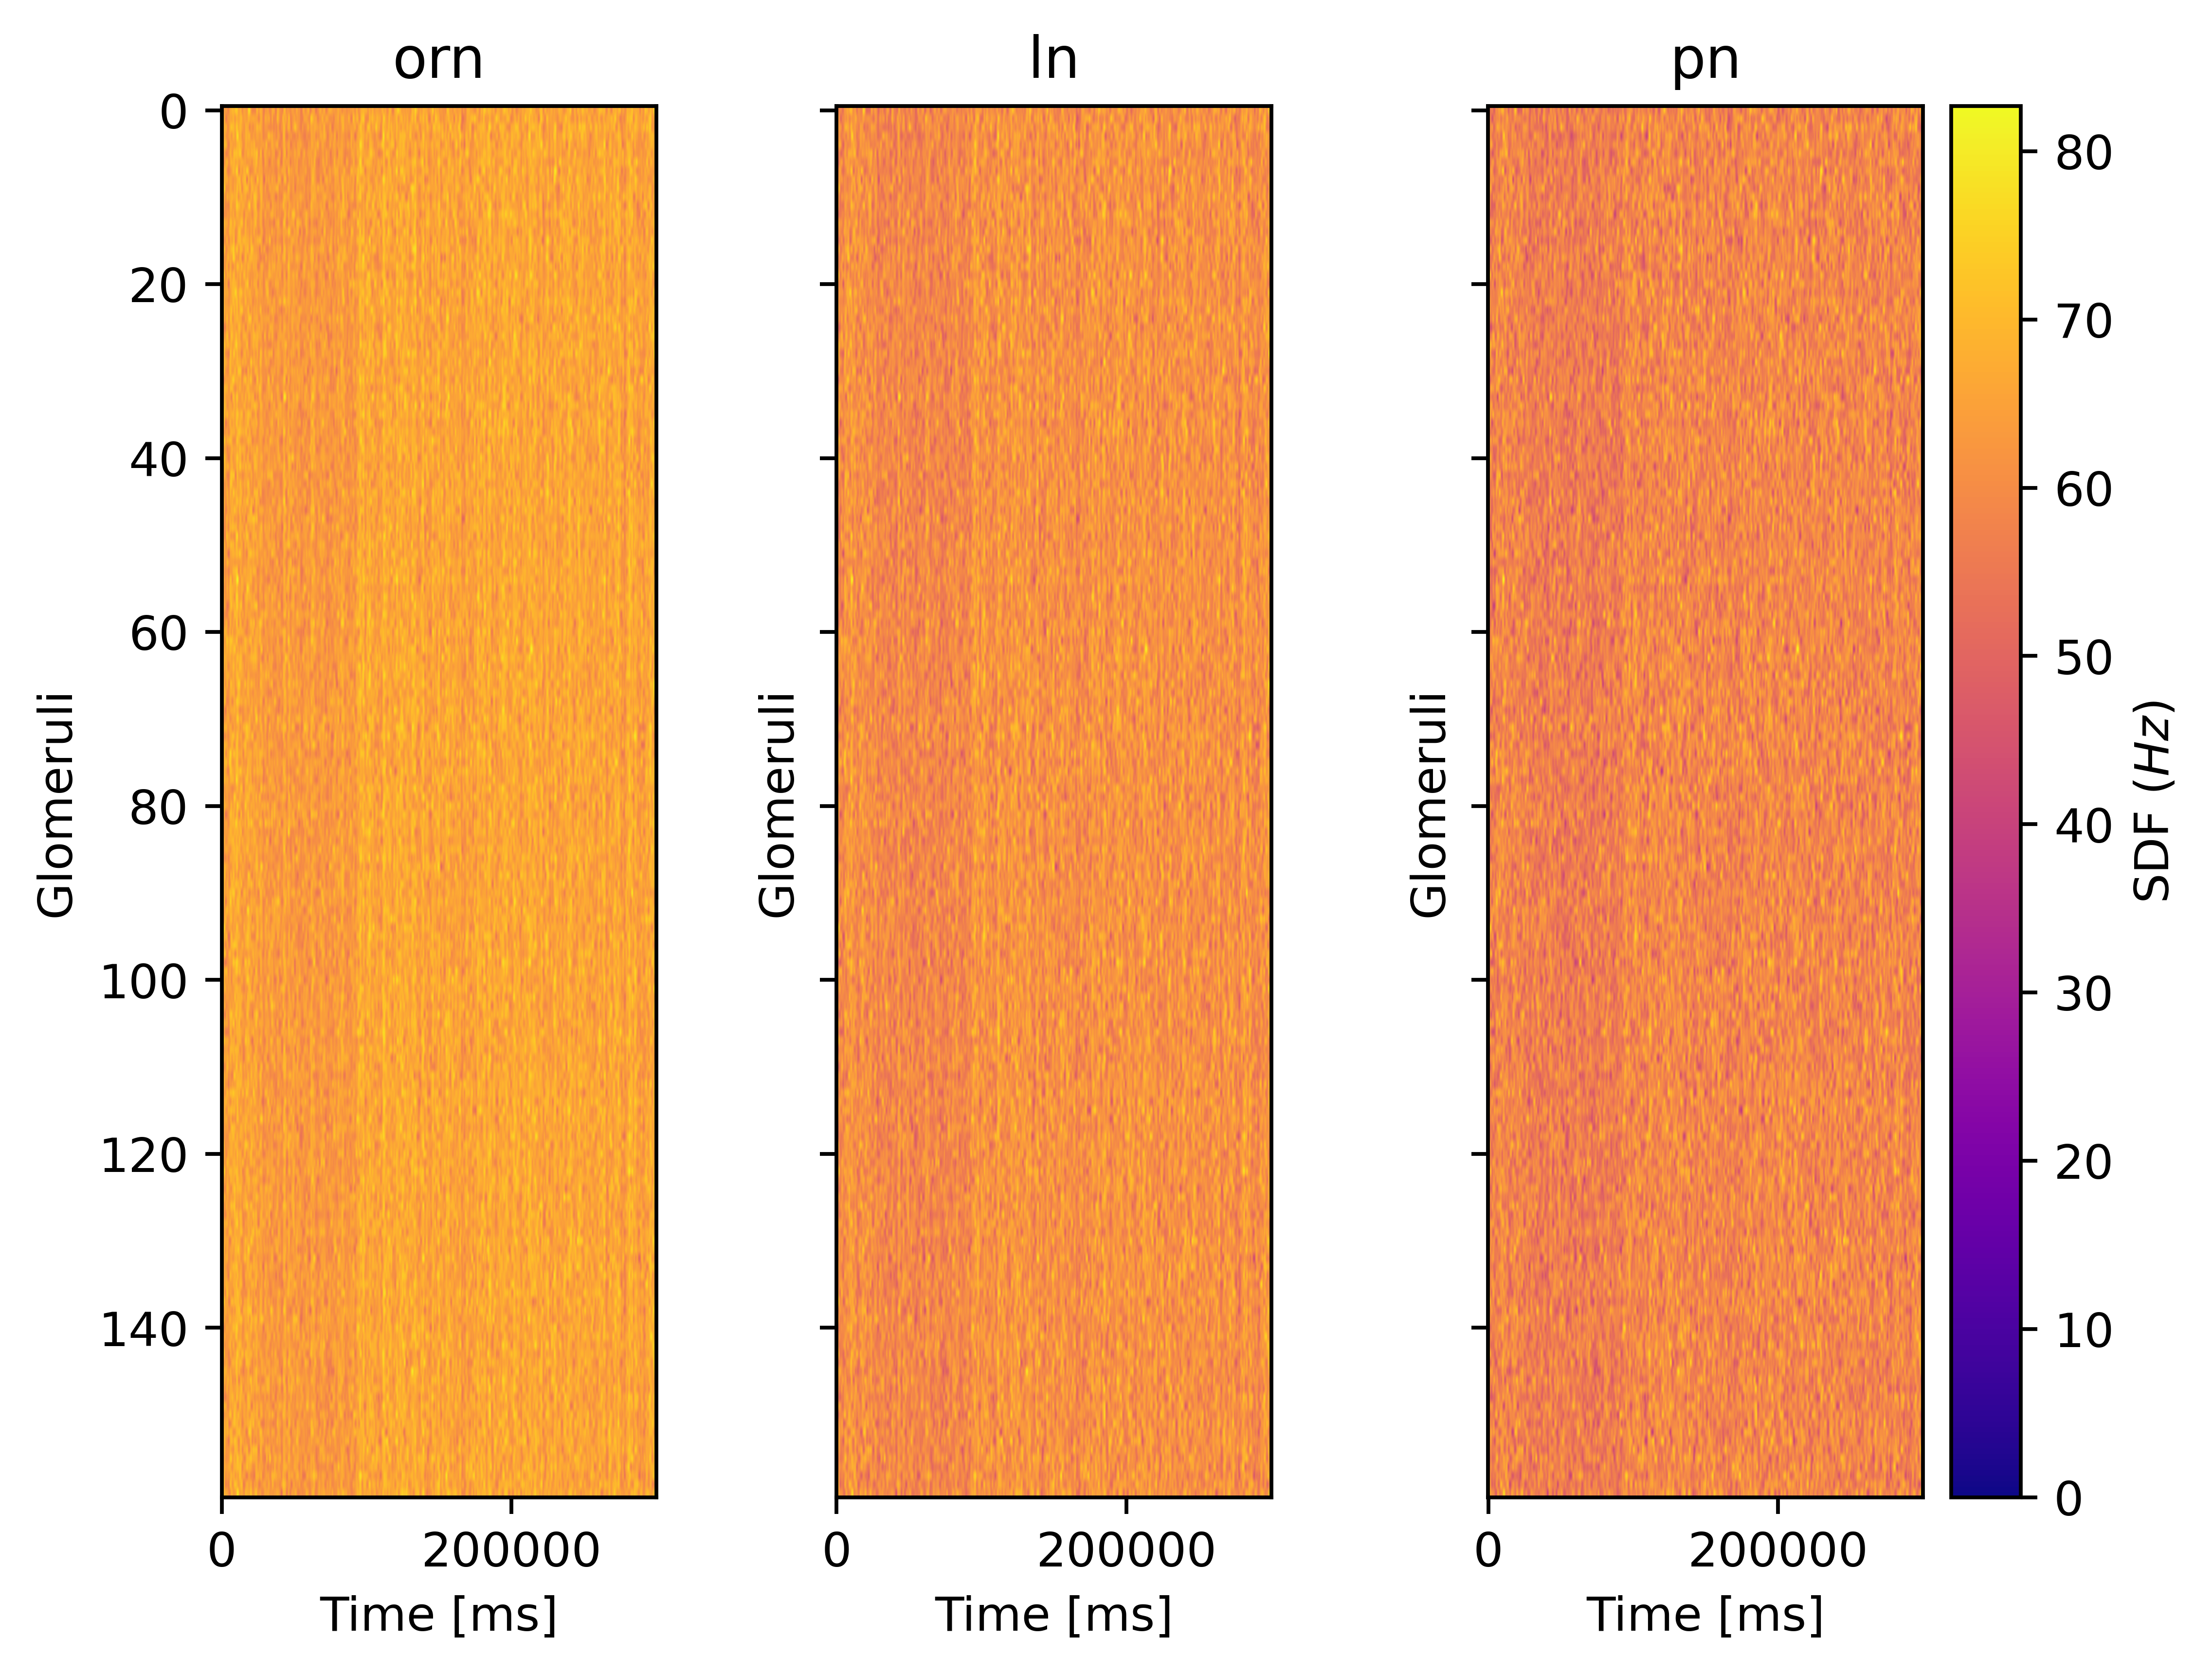
\includegraphics[width=\textwidth]{sdf-tenth-poisson}
    \caption{Tenth}
    \label{fig:sdf-tenth-poisson-finding-asleep}
  \end{subfigure}
  \begin{subfigure}[t]{0.5\textwidth}
    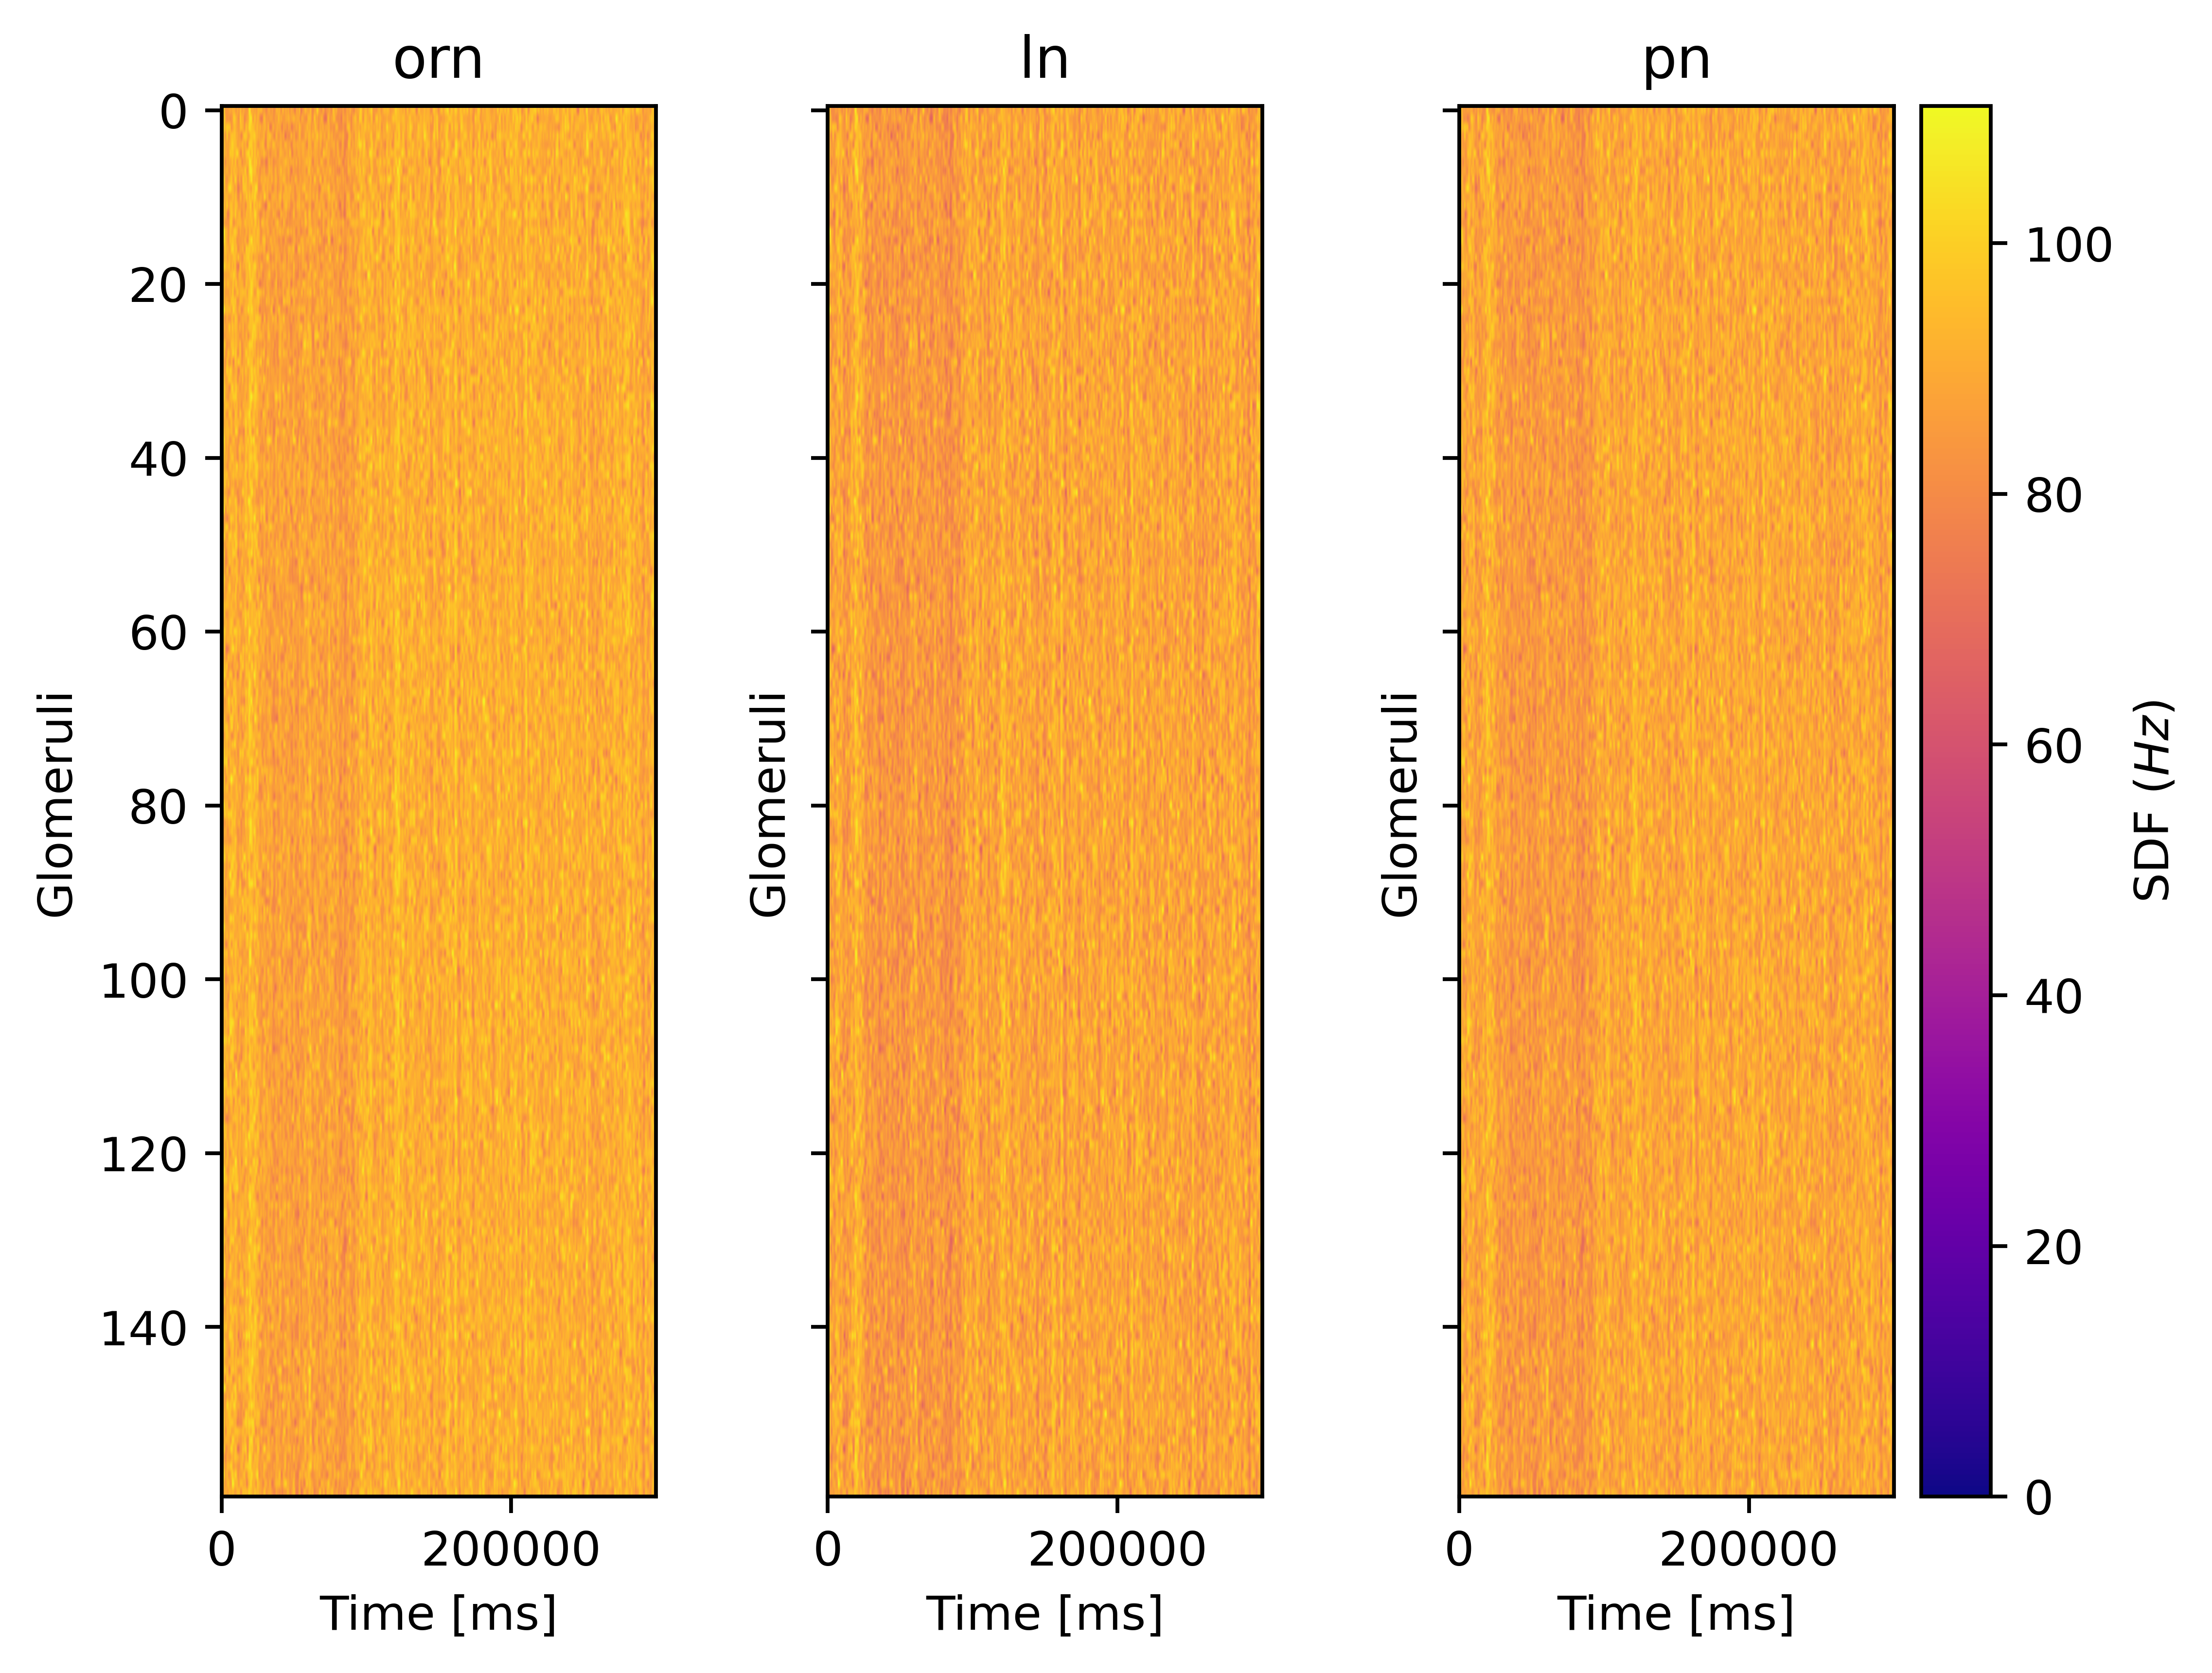
\includegraphics[width=\textwidth]{sdf-hundreth-poisson}
    \caption{Hundredth}
    \label{fig:sdf-hundredth-poisson-finding-asleep}
  \end{subfigure}
  \caption{Spike density matrix of the spontaneous activity of the antennal lobe with the Poisson trains and different reduction of the inhibitory synapses. $\SI{60}{\second}$ of simulation.}
  \label{fig:sdf-finding-asleep-2}
\end{figure}

The resulting spike density matrices are shown in figures \ref{fig:sdf-finding-asleep-1} and \ref{fig:sdf-finding-asleep-2}.
It can be noted how the coupling of the network increases as the inhibitory synapses are reduced.
In particular, it can be seen how the activity of the projection neurons increases and becomes increasingly similar to the one of the olfactory receptor neurons as the inhibitory synapses are reduced and becomes almost the same in the ``Hundredth'' simulation, suggesting that reducing the inhibitory synapses by a factor of $100$ makes their effect on the network negligible.\\
The same effect can be seen in the correlation matrices, shown in figures \ref{fig:correlation-finding-asleep-1} and \ref{fig:correlation-finding-asleep-2}.

\begin{figure}
  \begin{subfigure}[t]{\textwidth}
    \centering
    \includegraphics[width=\textwidth]{correlation-awake-no-poisson}
    \caption{Awake (without correlated input). Average correlation per population $\overline{Corr_{ORN}} = 0.006$, $\overline{Corr_{LN}} = 0.003$, $\overline{Corr_{PN}} = 0.001$}
    \label{fig:correlation-awake-poisson-finding-asleep}
  \end{subfigure}
  \begin{subfigure}[t]{\textwidth}
    \centering
    \includegraphics[width=\textwidth]{correlation-halved-poisson}
    \caption{Halved. Average correlation per population $\overline{Corr_{ORN}} = 0.32$, $\overline{Corr_{LN}} = 0.09$, $\overline{Corr_{PN}} = 0.01$}
    \label{fig:correlation-halved-poisson-finding-asleep}
  \end{subfigure}
  \begin{subfigure}[t]{\textwidth}
    \centering
    \includegraphics[width=\textwidth]{correlation-quarter-poisson}
    \caption{Quarter. Average correlation per population $\overline{Corr_{ORN}} = 0.31$, $\overline{Corr_{LN}} = 0.14$, $\overline{Corr_{PN}} = 0.009$}
    \label{fig:correlation-quarter-poisson-finding-asleep}
  \end{subfigure}
  \caption{Correlation of the spontaneous activity between glomeruli of the antennal lobe with the Poisson trains and different reduction of the inhibitory synapses. $\SI{60}{\second}$ of simulation.}
  \label{fig:correlation-finding-asleep-1}
\end{figure}

\begin{figure}
  \begin{subfigure}[t]{\textwidth}
    \centering
    \includegraphics[width=\textwidth]{correlation-tenth-poisson}
    \caption{Tenth. Average correlation per population $\overline{Corr_{ORN}} = 0.32$, $\overline{Corr_{LN}} = 0.22$, $\overline{Corr_{PN}} = 0.12$}
    \label{fig:correlation-tenth-poisson-finding-asleep}
  \end{subfigure}
  \begin{subfigure}[t]{\textwidth}
    \includegraphics[width=\textwidth]{correlation-hundreth-poisson}
    \caption{Hundredth. Average correlation per population $\overline{Corr_{ORN}} = 0.35$, $\overline{Corr_{LN}} = 0.32$, $\overline{Corr_{PN}} = 0.32$}
    \label{fig:correlation-quarter-poisson-finding-asleep}
  \end{subfigure}
  \caption{Correlation of the spontaneous activity between glomeruli of the antennal lobe with the Poisson trains and different reduction of the inhibitory synapses. $\SI{60}{\second}$ of simulation.}
  \label{fig:correlation-finding-asleep-2}
\end{figure}

From the correlation figures (\ref{fig:correlation-finding-asleep-1} and \ref{fig:correlation-finding-asleep-2}), it can be seen how the difference between the correlation of the olfactory receptor neurons and the projection neurons reduces with the inhibitory synapses strength (figure \ref{fig:correlation-change-normalized}).

\begin{figure}
  \centering
  \includegraphics[width=\textwidth]{change_in_correlation_asleep}
  \caption{Change in the difference in the correlation between olfactory receptor neurons and projection neurons in the different reduced synapses strenght conditions.}
  \label{fig:correlation-change-normalized}
\end{figure}

\begin{figure}
  \centering
  \includegraphics[width=\textwidth]{change_in_correlation_asleep_pn}
  \caption{Change in the correlation of projection neurons in the different reduced synapses strenght conditions.}
  \label{fig:correlation-change}
\end{figure}

Figure \ref{fig:correlation-change} shows the correlation between glomeruli in the projection neurons, averaged over several simulations.
It can be seen that there is a small decrease in correlation between the ``Halved'' and the ``Quarter'' simulation that can be ascribed to statistical error, while a kink is found in the ``Tenth'' simulation, suggesting that the inhibitory synapses stop to have a significant impact on the network already at a reduction factor of $10$.\\
Looking instead at figure \ref{fig:correlation-change-normalized}, the amount of correlation that it is lost due to the effect of the inhibitory synapses can be seen.
In particular, in the awake condition and in the ``Hundredth'' simulation almost no correlation is lost.
This is due to two different reason: in the awake condition there is no correlated input, while in the ``Hundredth'' the inhibitory synapses have stopped having an impact on the activity of the network.
Moreover it can be observed that this correlation difference decreases from the ``Halved'' to the Hundredth'', suggesting that the weaker the inhibitory synapses are, the less able the network is to filter out correlated input coming into the synapses.
From this it can be inferred that the inhibitory synapses decouple the activity of the olfactory receptor neurons and the projection neurons, and their effect is particularly significant when the input of the network presents a level of correlation.
The correlation change between the populations approaches zero in the ``Hundredth'' simulation, again supporting the fact that the inhibitory synapses are negligible in this condition.

\section{Comparison between awake and asleep states}
To find which of the different inhibitory synapses reduction is the best to simulate the asleep state, the features described in section \ref{sec:feature-extraction} are extracted from the different simulations and compared.
These features can be classified into two categories: one set of features will regard the distribution of the activity of the projection neurons, while the other set will regard the functional connectivity of the network.\\

\begin{figure}
  \centering
  \includegraphics[width=\textwidth]{experimental-feature-distribution}
  \caption{Distribution of the different features extracted from the awake and the asleep state, image from \cite{sleep-correlates}.}
  \label{fig:experimental-feature-distribution}
\end{figure}

Experimental results (shown in figure \ref{fig:experimental-feature-distribution}) suggest a shift in the distribution of the different features between the awake and the asleep state.
In particular, the different distributions of the features extracted from the asleep state suggest that the asleep state is characterized by a more strongly functionally connected network with greater variability.\\

\begin{figure}
  \centering
  \includegraphics[width=\textwidth]{normal-halved-feature-distribution}
  \caption{Distribution of the different features extracted from the normal and the halved simulation. Each point is extracted from a second of simulation.}
  \label{fig:normal-halved-feature-distribution}
\end{figure}

\begin{figure}
  \centering
  \includegraphics[width=\textwidth]{normal-quarter-feature-distribution}
  \caption{Distribution of the different features extracted from the normal and the quarter simulation. Each point is extracted from a second of simulation.}
  \label{fig:normal-quarter-feature-distribution}
\end{figure}

\begin{figure}
  \centering
  \includegraphics[width=\textwidth]{normal-tenth-feature-distribution}
  \caption{Distribution of the different features extracted from the normal and the tenth simulation. Each point is extracted from a second of simulation.}
  \label{fig:normal-tenth-feature-distribution}
\end{figure}

\begin{figure}
  \centering
  \includegraphics[width=\textwidth]{normal-hundreth-feature-distribution}
  \caption{Distribution of the different features extracted from the normal and the hundredth simulation. Each point is extracted from a second of simulation.}
  \label{fig:normal-hundreth-feature-distribution}
\end{figure}

The same features are extracted from the different simulations and compared with the ones extracted from the awake state (figures \ref{fig:normal-halved-feature-distribution}, \ref{fig:normal-quarter-feature-distribution}, \ref{fig:normal-tenth-feature-distribution} and \ref{fig:normal-hundreth-feature-distribution}).
The best fit to experimental data seems to be the one between the awake state and the ``Quarter'' simulation.\\
Something interesting that can be seen from the figures is that the difference in features between the different values of inhibitory synapses doesn't seem to change linearly with the change in inhibition.
This behavior is explored in figures \ref{fig:feature-distribution-behavior-1}, \ref{fig:feature-distribution-behavior-2}, \ref{fig:feature-distribution-behavior-3}, \ref{fig:feature-distribution-behavior-4}.
It can be seen how for all the features beside standard deviation (plot \ref{fig:std-evolution}), skewness (plot \ref{fig:skew-evolution}) and kurtosis (plot \ref{fig:kurtosis-evolution}) there is a change in directionality of the mean of the feature.
This non-linear effect suggests that, as expected, the inhibitory synapses perform a non-linear function in the network, changing how the input is represented.
Furthermore, there is no significant difference in features' means between the ``Tenth'' and ``Hundredth'' simulations, suggesting that the inhibitory synapses reduction by a factor of $10$ is great enough to make the local neurons unable to perform their function.\\
Beside betweenness and transitivity the non-linearity of the features seems to derive from the introduction of the correlated input in the simulations with reduced inhibitory synapses strenght.

\begin{figure}
  \begin{subfigure}[t]{0.48\textwidth}
    \centering
    \includegraphics[width=\textwidth]{std_evolution}
    \caption{Behavior of the standard deviation during the simulation of the different inhibitory synapses reduction. Reduction factor on the $x$-axis}
    \label{fig:std-evolution}
  \end{subfigure}
  \begin{subfigure}[t]{0.48\textwidth}
    \centering
    \includegraphics[width=\textwidth]{skew_evolution}
    \caption{Behavior of the skewness during the simulation of the different inhibitory synapses reduction. Reduction factor on the $x$-axis}
    \label{fig:skew-evolution}
  \end{subfigure}
  \begin{subfigure}[t]{\textwidth}
    \centering
    \includegraphics[width=0.5\textwidth]{kurtosis_evolution}
    \caption{Behavior of the kurtosis during the simulation of the different inhibitory synapses reduction. Reduction factor on the $x$-axis}
    \label{fig:kurtosis-evolution}
  \end{subfigure}
  \caption{Behavior of standard deviation, skewness and kurtosis during the simulation of the different inhibitory synapses reduction.}
  \label{fig:feature-distribution-behavior-1}
\end{figure}

\begin{figure}
  \begin{subfigure}[t]{0.48\textwidth}
    \centering
    \includegraphics[width=\textwidth]{sampen_evolution}
    \caption{Behavior of sample entropy during the simulation of the different inhibitory synapses reduction. Reduction factor on the $x$-axis}
    \label{fig:sampen-evolution}
  \end{subfigure}
  \begin{subfigure}[t]{0.48\textwidth}
    \centering
    \includegraphics[width=\textwidth]{hurst_rs_evolution}
    \caption{Behavior of the Hurst during the simulation of the different inhibitory synapses reduction. Reduction factor on the $x$-axis}
    \label{fig:hurst-evolution}
  \end{subfigure}
  \begin{subfigure}[t]{\textwidth}
    \centering
    \includegraphics[width=0.5\textwidth]{dfa_evolution}
    \caption{Behavior of the DFA during the simulation of the different inhibitory synapses reduction. Reduction factor on the $x$-axis}
    \label{fig:dfa-evolution}
  \end{subfigure}
  \caption{Behavior of sample entropy, Hurst and DFA during the simulation of the different inhibitory synapses reduction.}
  \label{fig:feature-distribution-behavior-2}
\end{figure}

\begin{figure}
  \begin{subfigure}[t]{0.48\textwidth}
    \centering
    \includegraphics[width=\textwidth]{betweenness_bin_evolution}
    \caption{Behavior of the betweenness during the simulation of the different inhibitory synapses reduction. Reduction factor on the $x$-axis}
    \label{fig:betweenness-evolution}
  \end{subfigure}
  \begin{subfigure}[t]{0.48\textwidth}
    \centering
    \includegraphics[width=\textwidth]{transitivity_bd_evolution}
    \caption{Behavior of the transitivity during the simulation of the different inhibitory synapses reduction. Reduction factor on the $x$-axis}
    \label{fig:transitivity-evolution}
  \end{subfigure}
  \begin{subfigure}[t]{\textwidth}
    \centering
    \includegraphics[width=0.5\textwidth]{degrees_dir_evolution}
    \caption{Behavior of the degree during the simulation of the different inhibitory synapses reduction.}
    \label{fig:degree-evolution}
  \end{subfigure}
  \caption{Behavior of betweenness, transitivity and degree during the simulation of the different inhibitory synapses reduction.}
  \label{fig:feature-distribution-behavior-3}
\end{figure}

\begin{figure}
  \begin{subfigure}[t]{0.48\textwidth}
    \centering
    \includegraphics[width=\textwidth]{efficiency_bin_evolution}
    \caption{Behavior of the efficiency during the simulation of the different inhibitory synapses reduction. Reduction factor on the $x$-axis}
    \label{fig:efficiency-evolution}
  \end{subfigure}
  \begin{subfigure}[t]{0.48\textwidth}
    \centering
    \includegraphics[width=\textwidth]{norm_evolution}
    \caption{Behavior of the Frobenius norm during the simulation of the different inhibitory synapses reduction. Reduction factor on the $x$-axis}
    \label{fig:norm-evolution}
  \end{subfigure}
  \caption{Behavior of efficiency and Frobenius norm during the simulation of the different inhibitory synapses reduction.}
  \label{fig:feature-distribution-behavior-4}
\end{figure}
